\documentclass[11pt]{article}
\usepackage[margin=0.8in]{geometry}
\usepackage[T1]{fontenc}
\usepackage[utf8]{inputenc}
\usepackage{booktabs,longtable,graphicx,url,array,microtype}
\setlength{\LTpre}{6pt}
\setlength{\LTpost}{6pt}
\setlength{\tabcolsep}{3pt}
\renewcommand{\arraystretch}{1.08}
\renewcommand{\thetable}{S\arabic{table}}
\renewcommand{\thefigure}{S\arabic{figure}}
\title{Supplementary Material for\\\emph{Timestep-Conditioned Adapter Scaling for Multi-view Diffusion Texture Generation}}
\author{Anonymous authors}
\date{}
\begin{document}
\maketitle
\noindent This supplement supports the revised 01549 manuscript. Fresh C is an image-space comparison on 300 UIDs disjoint from the original 01549 evaluation/probe IDs, the 1,118-object training list, and clean-v2 evaluation IDs. Its primary conditions and same-cohort addendum share one frozen adapter checkpoint, runner source, seed policy, inputs, target views, and metric implementation; the addendum is not an independent replication. Fresh C uses a controlled-retraining checkpoint and is not presented as a numerical reproduction of historical Table 4. Historical cohorts and interface checks are reported separately. Object is the inferential unit; multiple views and wrapper records do not increase $N$.

\section*{S1. Figure asset credits and selection status}
Main Figures~4--7 use Fresh C reference and method-level RGB outputs in a compact context-plus-shared-ROI layout. The original six-view, seven-condition panels remain in Supplementary Figure~S1. The selected examples are outcome-ranked illustrations, not a representative sample. Image, checkpoint, run, seed, ROI, and output hashes are listed in \texttt{FRESH\_C\_FIGURE\_SOURCE\_ROI\_MANIFEST.csv}.

The Fresh C No Adapter condition suppresses geometry-adapter correction. In the MVPainter wrapper, when \texttt{\_adapter\_scale} is unset the geometry residual is applied without a scale multiplier. These are different settings: No Adapter is not a rendered comparison against the unmodified native-default adapter path. Fresh C contains no separate output for that native-default path, so this part of the R1.1 request remains partially unresolved.

The current rights ledger records the selected Fresh C assets below as CC Attribution (CC BY 4.0), with figure use allowed when attributed. The complete credit line for each use is:
\begin{longtable}{p{4.3cm}p{10.9cm}}
\caption{Attribution for selected Fresh C assets in main Figures~5--7 and Supplementary Figure~S1.}\label{tab:supp-credits}\\
\toprule Use & Full attribution \\
\midrule\endfirsthead
\toprule Use & Full attribution \\
\midrule\endhead
Figure 7(a), C3--GFL endpoint-favourable example & \emph{Building 03} by Shalmon, via Sketchfab (\url{https://sketchfab.com/3d-models/c76ac44df995482185077da81939b306}), licensed CC BY 4.0 (\url{https://creativecommons.org/licenses/by/4.0/}). Fresh C target-view RGB outputs are cropped to the same ROI and arranged without color or detail adjustment. \\
Figure 5(a), C3-versus-fixed-scale example & \emph{Octaèdre} by Segolene Delamare, via Sketchfab (\url{https://sketchfab.com/3d-models/0571e6db30c84b1593bc55a8e145a430}), licensed CC BY 4.0 (\url{https://creativecommons.org/licenses/by/4.0/}). Fresh C target-view RGB outputs are cropped to the same ROI and arranged without color or detail adjustment. \\
Figure 5(b), Generic Linear counterexample & \emph{Cube 01} by b0rF4x, via Sketchfab (\url{https://sketchfab.com/3d-models/06fa4974f8cd4d4ea792e98fa1521457}), licensed CC BY 4.0 (\url{https://creativecommons.org/licenses/by/4.0/}). Fresh C target-view RGB outputs are cropped to the same ROI and arranged without color or detail adjustment. \\
Figure 7(b) and Figure S1(a), adverse C3--GFL example & \emph{Boat Low Poly Game Ready} by INinja, via Sketchfab (\url{https://sketchfab.com/3d-models/d0e116a62bfc4cdd9edf60671073b306}), licensed CC BY 4.0 (\url{https://creativecommons.org/licenses/by/4.0/}). Fresh C target-view RGB outputs are cropped to the same ROI and arranged without color or detail adjustment. \\
Figure 6, selected Fresh C color/detail illustration & \emph{E5-5-2} by artsiyu, via Sketchfab (\url{https://sketchfab.com/3d-models/f6979d7ff8e54c4daf00fee46f09a139}), licensed CC BY 4.0 (\url{https://creativecommons.org/licenses/by/4.0/}). This previously viewed object came from a pre-existing C3--GFL FG-LPIPS stratum and was not selected for color. \\
\bottomrule
\end{longtable}

\section*{S2. Complete Fresh C paired image-space statistics}
Table~\ref{tab:supp-freshc} reports the complete seven-endpoint paired results for C3--GFL and each of the three named addendum contrasts. The primary C3--GFL FG-PSNR result is unadjusted as the single registered primary endpoint. The six registered secondary C3--GFL endpoints use their Holm family. The addendum's FG-PSNR and FG-LPIPS contrasts use the frozen six-test primary family; the other five endpoints per contrast use the separate 15-test secondary Core-7 family. All contrasts are mean A-minus-B differences with 10,000 object bootstrap resamples and pointwise two-sided percentile 95\% CIs. Positive values favour A for PSNR/SSIM; negative values favour A for LPIPS. Adjusted $p$-values are from the frozen analysis authority. “A favourable” is the fraction of object-level differences in A's favourable direction and is descriptive.

\begingroup\scriptsize
\begin{longtable}{p{2.5cm}p{4.0cm}p{1.5cm}p{1.5cm}p{1.6cm}}
\caption{Complete paired object-level image-space results for the primary C3--GFL contrast and the three named same-cohort addendum contrasts. Differences are A minus B; favorable-object percentages respect endpoint direction.}\label{tab:supp-freshc}\\
\toprule
Endpoint & Mean difference [95\% CI] & Median & A favorable & Adjusted $p$ \\
\midrule
\endfirsthead
\toprule Endpoint & Mean difference [95\% CI] & Median & A favorable & Adjusted $p$ \\
\midrule\endhead
\multicolumn{5}{l}{\textbf{C3 minus GFL}}\\
FG-PSNR (dB) & +0.522 [+0.404, +0.641] & +0.555 & 68.7\% & primary \\
FG-LPIPS & -0.005345 [-0.006326, -0.004403] & -0.004547 & 71.0\% & $3.2\times 10^{-22}$ \\
FG-SSIM & +0.02453 [+0.02120, +0.02805] & +0.02004 & 84.3\% & $5.9\times 10^{-33}$ \\
Edge-SSIM & +0.004494 [+0.003411, +0.005586] & +0.003613 & 69.0\% & $9.4\times 10^{-14}$ \\
Full-view PSNR (dB) & +0.271 [+0.170, +0.373] & +0.220 & 59.3\% & $4\times 10^{-07}$ \\
Full-view LPIPS & -0.003880 [-0.004926, -0.002873] & -0.003029 & 64.3\% & $8\times 10^{-13}$ \\
Full-view SSIM & +0.005619 [+0.004627, +0.006704] & +0.005205 & 83.0\% & $7.9\times 10^{-22}$ \\
\multicolumn{5}{l}{\textbf{C3 minus Generic Linear}}\\
FG-PSNR (dB) & -0.593 [-0.837, -0.351] & +0.074 & 51.7\% & $7.2\times 10^{-06}$ \\
FG-LPIPS & +0.013512 [+0.011601, +0.015487] & +0.012229 & 25.7\% & $1.3\times 10^{-32}$ \\
FG-SSIM & -0.02810 [-0.03197, -0.02439] & -0.02521 & 20.0\% & $2.9\times 10^{-35}$ \\
Edge-SSIM & -0.010693 [-0.013004, -0.008495] & -0.008967 & 33.7\% & $1.6\times 10^{-17}$ \\
Full-view PSNR (dB) & -0.503 [-0.686, -0.322] & -0.139 & 46.7\% & $2.7\times 10^{-07}$ \\
Full-view LPIPS & -0.000897 [-0.002578, +0.000862] & -0.001307 & 54.3\% & $0.611$ \\
Full-view SSIM & +0.000046 [-0.000984, +0.001011] & +0.001213 & 57.0\% & $0.927$ \\
\multicolumn{5}{l}{\textbf{LLH minus C3}}\\
FG-PSNR (dB) & +0.621 [+0.391, +0.855] & -0.153 & 46.7\% & $1.2\times 10^{-06}$ \\
FG-LPIPS & -0.012140 [-0.013861, -0.010480] & -0.010837 & 75.0\% & $9\times 10^{-34}$ \\
FG-SSIM & +0.01658 [+0.01311, +0.02003] & +0.01307 & 67.0\% & $9\times 10^{-18}$ \\
Edge-SSIM & +0.009033 [+0.006867, +0.011296] & +0.006741 & 63.3\% & $2.3\times 10^{-13}$ \\
Full-view PSNR (dB) & +0.816 [+0.639, +0.998] & +0.419 & 59.3\% & $3.2\times 10^{-16}$ \\
Full-view LPIPS & +0.004909 [+0.003266, +0.006510] & +0.004538 & 36.7\% & $3.5\times 10^{-08}$ \\
Full-view SSIM & -0.004330 [-0.005176, -0.003482] & -0.004563 & 27.7\% & $5.9\times 10^{-20}$ \\
\multicolumn{5}{l}{\textbf{LLH minus Generic Linear}}\\
FG-PSNR (dB) & +0.028 [-0.015, +0.070] & +0.017 & 52.3\% & $0.201$ \\
FG-LPIPS & +0.001372 [+0.000762, +0.002081] & +0.000176 & 46.7\% & $0.000114$ \\
FG-SSIM & -0.01152 [-0.01337, -0.00996] & -0.00945 & 8.0\% & $2.6\times 10^{-31}$ \\
Edge-SSIM & -0.001660 [-0.002096, -0.001256] & -0.001648 & 27.3\% & $1.2\times 10^{-12}$ \\
Full-view PSNR (dB) & +0.313 [+0.278, +0.347] & +0.304 & 87.3\% & $2\times 10^{-47}$ \\
Full-view LPIPS & +0.004011 [+0.003390, +0.004684] & +0.003904 & 18.0\% & $1.7\times 10^{-26}$ \\
Full-view SSIM & -0.004284 [-0.005217, -0.003543] & -0.003432 & 5.7\% & $8.5\times 10^{-20}$ \\
\bottomrule
\end{longtable}

\endgroup

\section*{S3. Supporting layer/window and schedule evidence}
A2 is exploratory discovery evidence; A3 is a higher-dose stress regime on the same underlying cohort. A3b is a bounded Fresh B layer/window analysis. Object-cluster tests detect response heterogeneity under the tested interventions, but they do not identify a dose-independent layer-by-time mechanism or an optimal schedule.

\begin{table}[ht]
\centering\small
\caption{Object-cluster Wald interaction summaries for the tested layer-by-window maps. Cell RMSE and interaction share describe these observed maps; they are not causal effect sizes.}\label{tab:supp-layerwindow}
\begin{tabular}{lp{2.1cm}rp{4.2cm}p{2.6cm}}\toprule Map & Endpoint & Wald statistic & Interaction share; cell RMSE & Wald $p$ (A3b Holm) \\\midrule
A2 & FG-LPIPS & 481.081 & 43.5\%; 0.001695 & $8.04\times10^{-99}$ \\
A2 & FG-PSNR & 1879.963 & 56.8\%; 0.1222 dB & $<10^{-300}$ \\
A3 & FG-LPIPS & 657.237 & 11.9\%; 0.00643 & $1.14\times10^{-136}$ \\
A3 & FG-PSNR & 1389.118 & 0.8\%; 0.207 dB & $1.28\times10^{-294}$ \\
A3b & FG-LPIPS & 225.015 & 14.0\%; 0.000342 & $5.37\times10^{-43}$ \\
A3b & FG-PSNR & 525.700 & 36.0\%; 0.0205 dB & $3.43\times10^{-107}$ \\
\bottomrule\end{tabular}
\end{table}

The earlier A3b common-support calculation compared 10-step integrated raw $L_2$ norms across three layer groups. Because the saved correction tensors have different spatial resolutions (24$\times$16, 48$\times$32, and 96$\times$64) and the traces omit channel counts, absolute norms are dimension-dependent across groups. We withdraw the central-90\% intervals and 0/2,250 overlap as cross-group dose-support evidence. The earlier development calibration also used cross-layer raw $L_2$ and is not interpreted as equal-dose targeting. The fixed A3b scale values remain the tested bounded profiles. A3b remains retrospective sensitivity evidence: its map describes response heterogeneity under the tested interventions, but does not identify a dose-independent layer-by-window effect.

The separate Fresh B cohort ($N=150$) supplies schedule-location context for LLH, not evidence for C3. Table~\ref{tab:supp-freshb} preserves both registered LLH comparisons and the post-outcome HLL--LLL diagnostic. Paired intervals use 10,000 object-bootstrap resamples (seed 20261002). The LLH--LFM-EXACT intervals lie within the protocol's practical margins (FG-PSNR $\pm0.5$ dB; FG-LPIPS $\pm0.01$); this is a budget-explained interpretation within those margins, not exact equality. HLL--LLL is exploratory and its endpoint directions differ.

The Fresh B protocol-lock file states a freeze time of 2026-10-05 08:40 UTC, while the earliest preserved commit containing that file is dated 2026-10-06 00:52 UTC; its parent does not contain the file. This history does not establish when the lock was first created outside Git, but it cannot authenticate pre-run availability. Accordingly, Fresh B temporal contrasts, the A3b map, and the post-lock generic extension are treated as retrospective sensitivity evidence in this paper, even where their calculations follow the recorded comparison family. They are not described as verified preregistered confirmation.

\begin{table}[ht]
\centering\small
\caption{Fresh B paired object-level LLH comparisons, classified here as retrospective sensitivity because pre-run lock availability cannot be authenticated from the preserved history. Effects are A minus B; favorable rates respect endpoint direction. Holm values reproduce the recorded family.}\label{tab:supp-freshb}
\begin{tabular}{p{3.7cm}p{1.7cm}p{5.7cm}p{1.4cm}p{2.2cm}}\toprule Contrast & Endpoint & Mean [95\% CI] & A favors & $p$ / status \\\midrule
LLH--LFM-EXACT & FG-PSNR & +0.325 [+0.209,+0.446] dB & 54.0\% & raw $\leq0.0001$ \\
LLH--LFM-EXACT & FG-LPIPS & $-0.00460$ [$-0.00563,-0.00357$] & 76.0\% & raw $\leq0.0001$ \\
LLH--HLL & FG-PSNR & +0.687 [+0.404,+0.981] dB & 45.3\% & $\leq0.0004$; median $-0.104$ dB \\
LLH--HLL & FG-LPIPS & $-0.01098$ [$-0.01349,-0.00851$] & 80.7\% & $\leq0.0004$ \\
LLH--LLL & FG-PSNR & +0.734 [+0.597,+0.875] dB & 79.3\% & $\leq0.0004$ \\
LLH--LLL & FG-LPIPS & $-0.00845$ [$-0.01029,-0.00659$] & 82.0\% & $\leq0.0004$ \\
HLL--LLL (exploratory) & FG-PSNR & +0.047 [$-0.120,+0.208$] dB & 66.0\% & 0.5696; median +0.476 dB \\
HLL--LLL (exploratory) & FG-LPIPS & +0.00253 [+0.00155,+0.00354] & 40.0\% & $\leq0.0002$; median +0.00139 \\
\bottomrule\end{tabular}
\end{table}

The post-lock generic-schedule extension on this same Fresh B cohort is a retrospective sensitivity analysis, not independent confirmation. Table~\ref{tab:supp-generic} reports the recorded budget-matched comparisons and endpoint-matched linear counter-result. Nominal requested-scale means do not equalize post-scale residual dose; these LLH comparisons do not establish dose-adjusted schedule superiority or strengthen C3 specifically.

\clearpage
\begingroup\scriptsize
\begin{longtable}{p{3.4cm}p{1.7cm}p{4.4cm}p{1.3cm}p{2.4cm}}
\caption{Post-lock Fresh B generic-schedule extension (same $N=150$ cohort). Effects are LLH minus comparator. Budget-matched schedules form the locked eight-schedule family; endpoint-matched linear is the registered counter-comparison.}\label{tab:supp-generic}\\
\toprule Contrast & Endpoint & Mean [95\% CI] & A favors & Holm $p$ \\
\midrule\endfirsthead
\toprule Contrast & Endpoint & Mean [95\% CI] & A favors & Holm $p$ \\
\midrule\endhead
LLH--budget linear & FG-PSNR & +0.0967 [+0.0594,+0.1357] dB & 65.3\% & Holm $p\leq0.0008$ \\
LLH--budget linear & FG-LPIPS & -0.0009 [-0.0013,-0.0004] & 65.3\% & Holm $p=0.0008$ \\
LLH--budget cosine & FG-PSNR & +0.4629 [+0.3526,+0.5780] dB & 74.7\% & Holm $p\leq0.0008$ \\
LLH--budget cosine & FG-LPIPS & -0.0059 [-0.0071,-0.0046] & 80.0\% & Holm $p\leq0.0008$ \\
LLH--budget trapezoid & FG-PSNR & +0.4404 [+0.3334,+0.5521] dB & 74.0\% & Holm $p\leq0.0008$ \\
LLH--budget trapezoid & FG-LPIPS & -0.0057 [-0.0070,-0.0045] & 78.0\% & Holm $p\leq0.0008$ \\
LLH--budget Gaussian & FG-PSNR & +0.4711 [+0.3584,+0.5892] dB & 74.7\% & Holm $p\leq0.0008$ \\
LLH--budget Gaussian & FG-LPIPS & -0.0058 [-0.0071,-0.0045] & 79.3\% & Holm $p\leq0.0008$ \\
LLH--endpoint linear & FG-PSNR & -0.0373 [-0.0829,+0.0086] dB & -- & Holm $p=0.1150$ \\
LLH--endpoint linear & FG-LPIPS & +0.00109 [+0.0004,+0.0019] & -- & Holm $p=0.0024$ \\
\bottomrule
\end{longtable}
\endgroup

\clearpage
\section*{S4. Requested/applied scale and residual-correction accounting}
Table~\ref{tab:supp-execution} lists representative Fresh C C3 records at five denoising steps. The native caps are 3.0 (deep), 3.5 (middle), and 0.8 (shallow). A cap-active fraction of 100\% means all logged records in that group/step were clipped. Raw correction $L_2$ depends on both the residual and tensor dimensions, so it is not compared across layer groups. The table instead reports the median of wrapper-level mean absolute entries, a dimension-normalized descriptive summary; differences in feature scales and distributions still prevent interpreting it as an equal-dose intervention or quality outcome. The 750-row source accounting table contains all 50 steps, three groups, and five strategies.

\begingroup\scriptsize
\begin{longtable}{c l c c c r}
\caption{Representative Fresh C requested/applied scale and post-scale residual-correction accounting. The final column is the median wrapper-level mean absolute correction entry; it is dimension-normalized but remains descriptive. Wrappers, objects, and timesteps are not independent experimental units.}\label{tab:supp-execution}\\
\toprule Step & Layer group & Requested & Applied & Cap active & Median per-wrapper mean $|c|$ \\
\midrule\endfirsthead
\toprule Step & Layer group & Requested & Applied & Cap active & Median per-wrapper mean $|c|$ \\
\midrule\endhead
0 & Deep & 1.25 & 1.25 & 0\% & 1.4786 \\
0 & Middle & 1.25 & 1.25 & 0\% & 0.3540 \\
0 & Shallow & 1.25 & 0.80 & 100\% & 0.0128 \\
12 & Deep & 1.25 & 1.25 & 0\% & 1.3969 \\
12 & Middle & 1.25 & 1.25 & 0\% & 0.4881 \\
12 & Shallow & 1.25 & 0.80 & 100\% & 0.0151 \\
24 & Deep & 2.50 & 2.50 & 0\% & 2.2588 \\
24 & Middle & 2.50 & 2.50 & 0\% & 1.1408 \\
24 & Shallow & 2.50 & 0.80 & 100\% & 0.0169 \\
37 & Deep & 1.25 & 1.25 & 0\% & 0.7513 \\
37 & Middle & 1.25 & 1.25 & 0\% & 0.4596 \\
37 & Shallow & 1.25 & 0.80 & 100\% & 0.0176 \\
49 & Deep & 1.25 & 1.25 & 0\% & 0.7354 \\
49 & Middle & 1.25 & 1.25 & 0\% & 0.1459 \\
49 & Shallow & 1.25 & 0.80 & 100\% & 0.0116 \\
\bottomrule
\end{longtable}

\endgroup

\section*{S5. Historical and cross-interface boundaries}
The completed \texttt{MAIN-STAGE-276} follow-up contains 1,104 records (276 objects by four schedules), with 50 Euler steps, seed 42, unique-six target views, shared initial latents, and a common runner within the run. Its final run manifest records completion with exit code 0. The follow-up was specified after inspection of earlier clean-v2 results and was not blind. It is reported separately from Fresh C and is not an independent replication of the original 01549 development probe.

Here, temporal L--L--H means that the requested values are low in early and middle steps and high in late steps. This is distinct from the layer-conditioned Fresh C LLH addendum condition described in the main paper. With 50 steps, the code assigns 17/16/17 steps to early/middle/late. C3 therefore has deep/middle applied-scale sums of 82.5; temporal L--L--H has 83.75 because its high stage occupies 17 rather than 16 steps; the shallow applied sum is 40 for both after the 0.8 cap. The fixed-mean comparator has a deep/middle sum of 83.33 and a shallow sum of 40. These are near-matched scalar sums, not exactly equal sums or matched residual-norm doses.

Table~\ref{tab:supp-stage-placement} gives all six formal paired endpoints for C3 versus temporal L--L--H and C3 versus the fixed-mean comparator. Effects are C3 minus comparator; positive values favor C3 for PSNR/SSIM, and negative values favor C3 for LPIPS. Temporal L--L--H outperforms C3 on all six formal endpoints in this post-inspection stage-placement experiment: it has higher PSNR/SSIM and lower LPIPS endpoints. In contrast, C3 exceeds fixed-mean on five of six formal endpoints. These results show that the measured response varies with tested stage placement; they do not establish a universal schedule winner. The contrasts do not isolate placement from the small applied-scale-sum differences or the resulting residual-state trajectory, and post-scale residual norms are not matched.

\begin{longtable}{p{3.0cm}p{2.6cm}p{5.8cm}}
\caption{Formal paired comparisons from the strict-276 stage-placement follow-up. Effects are C3 minus comparator; 95\% percentile-bootstrap intervals are object-level.}\label{tab:supp-stage-placement}\\
\toprule Contrast & Endpoint & Mean difference [95\% CI] \\
\midrule\endfirsthead
\toprule Contrast & Endpoint & Mean difference [95\% CI] \\
\midrule\endhead
\multicolumn{3}{l}{\textbf{C3 minus temporal L--L--H}}\\
 & Full-view PSNR (dB) & $-0.268100$ [$-0.311101,-0.227797$] \\
 & FG-PSNR (dB) & $-0.177084$ [$-0.230539,-0.130784$] \\
 & FG-SSIM & $-0.008851$ [$-0.011455,-0.006291$] \\
 & Edge-SSIM & $-0.035301$ [$-0.036581,-0.034031$] \\
 & FG-LPIPS & $+0.001896$ [$+0.001205,+0.002578$] \\
 & Full-view LPIPS & $+0.008658$ [$+0.007465,+0.009831$] \\
\multicolumn{3}{l}{\textbf{C3 minus fixed-mean}}\\
 & Full-view PSNR (dB) & $+0.556369$ [$+0.525520,+0.589220$] \\
 & FG-PSNR (dB) & $+0.502875$ [$+0.462018,+0.542244$] \\
 & FG-SSIM & $+0.032083$ [$+0.028966,+0.035172$] \\
 & Edge-SSIM & $+0.001696$ [$+0.000611,+0.002782$] \\
 & FG-LPIPS & $-0.003797$ [$-0.004341,-0.003260$] \\
 & Full-view LPIPS & $+0.001420$ [$+0.000778,+0.002072$] \\
\bottomrule
\end{longtable}

The saved-artifact Full-SSIM branch is kept separate from the formal pre-save metrics above: C3 minus temporal L--L--H is $-0.001697$ (95\% CI [$-0.002047,-0.001340$]); C3 minus fixed-mean is $+0.007486$ ([$+0.006736,+0.008262$]). These saved-artifact values are not pooled with the formal metric column.

A retrospective strict-276 Core-7 summary uses the clean-v2 object list (SHA-256 \texttt{a6aa8ab6\allowbreak{}e475763e\allowbreak{}1b5e67dc\allowbreak{}8c712ec8\allowbreak{}f1940e39\allowbreak{}52d65897\allowbreak{}c8208875\allowbreak{}54bbd044}) and the same recorded checkpoint SHA as Fresh C. It shares the 276-object cohort/checkpoint lineage with the separate \texttt{MAIN-STAGE-276} profile-placement follow-up, so those results are not independent cohort replications. The row audit verifies 276 unique object indices per condition and identical object labels by index. However, Core-7 does not establish one common runner or fully shared inputs across all seven conditions: No Adapter and GFH are the two newly rerun arms with per-object input-tensor hashes; their recorded runner hash is \texttt{ae5d5664\allowbreak{}e7d0ebcd\allowbreak{}4bd84c7c\allowbreak{}7d688c4a\allowbreak{}8962c6d7\allowbreak{}4463fe88\allowbreak{}e7a86640\allowbreak{}4911e7e0}. C3 records a different runner hash, \texttt{d4af0c1d\allowbreak{}7f42168a\allowbreak{}585b505a\allowbreak{}6d775ea3\allowbreak{}ff7ffb18\allowbreak{}345156eb\allowbreak{}f358f272\allowbreak{}025fa7f2}; GFL and the three layer conditions do not establish the same runner hash, and their serialized rows do not contain per-object input-tensor hashes. Thus Core-7 is a retrospective diagnostic, not a same-runner confirmatory comparison. It is not pooled with Fresh C, and the shared checkpoint hash does not make it a numerical reproduction of the original 01549 Table 4 result.

Table~\ref{tab:supp-core7-means} gives the seven-condition means for the requested image-space endpoints. These stored metrics show an endpoint trade-off: C3 has a higher Full-view PSNR mean than GFH but a lower FG-PSNR mean. The Core-7 Layer LLH row is distinct from Fresh C's layer-conditioned LLH addendum and Fresh B's temporal LLH condition. Table~\ref{tab:supp-core7-contrasts} reports selected object-indexed contrasts. C3--GFH intervals were recalculated from the serialized per-object rows after inspection of the Core-7 summary; they are post-hoc, nominal pointwise intervals. The other listed contrasts reproduce the separate Core-7 paired-statistics file. The intervals describe the saved metric rows and do not overcome the common-runner/input-hash limitations.

\begin{table}[ht]
\centering\scriptsize\setlength{\tabcolsep}{4pt}
\caption{Retrospective Core-7 strict-276 condition means. Rows contain 276 object-level metrics per condition. The collection has incomplete common runner/input identity as described above; means are descriptive and are not Fresh C or an independently verified same-runner comparison.}
\label{tab:supp-core7-means}
\begin{tabular}{lccccc}\toprule
Condition & Full-view PSNR$\uparrow$ & FG-PSNR$\uparrow$ & FG-LPIPS$\downarrow$ & FG-SSIM$\uparrow$ & Edge-SSIM$\uparrow$ \\
\midrule
No Adapter & 10.563 & 8.826 & 0.2059 & 0.4799 & 0.4794 \\
GFL & 18.229 & 10.731 & 0.1917 & 0.3987 & 0.5201 \\
GFH & 18.242 & 13.153 & 0.1677 & 0.4783 & 0.5538 \\
C3 & 18.968 & 11.939 & 0.1817 & 0.4296 & 0.5278 \\
Layer Fixed Mean & 19.516 & 13.100 & 0.1698 & 0.4550 & 0.5363 \\
Layer LHL & 19.635 & 12.974 & 0.1719 & 0.4445 & 0.5273 \\
Layer LLH & 20.828 & 13.975 & 0.1610 & 0.4620 & 0.5476 \\
\bottomrule\end{tabular}
\end{table}

\begin{table}[ht]
\centering\small
\caption{Selected retrospective Core-7 paired contrasts (first condition minus second). Intervals are pointwise 95\% object-bootstrap percentile intervals with 10,000 resamples and seed 20260930; they are unadjusted and descriptive. The C3--GFH intervals were recalculated post hoc. The final column counts objects where the first condition is favorable for PSNR.}
\label{tab:supp-core7-contrasts}
\begin{tabular}{llcc}\toprule
Contrast & Endpoint & Mean difference [95\% CI] (dB) & Objects favoring first \\
\midrule
C3--GFH & Full-view PSNR & $+0.725229$ [$+0.647134,+0.806467$] & 240/276 \\
C3--GFH & FG-PSNR & $-1.214235$ [$-1.313952,-1.114705$] & 25/276 \\
C3--GFL & FG-PSNR & $+1.207771$ [$+1.116967,+1.294989$] & 259/276 \\
LLH--GFH & FG-PSNR & $+0.822292$ [$+0.616795,+1.033035$] & 148/276 \\
LLH--C3 & FG-PSNR & $+2.036527$ [$+1.806804,+2.260756$] & 227/276 \\
\bottomrule\end{tabular}
\end{table}

The frozen MV-Adapter layer/window probe analyzed 98 of 99 planned objects; the omitted input was a GLB with path geometry and no triangle faces, so no substitute was used. Its production additive-residual bootstrap had an invalid null and is not used for interaction inference. The post hoc object-cluster robust Wald reanalysis found no interaction surviving its exploratory four-metric Holm correction (FG-LPIPS Holm $p=0.303$; PSNR $p=0.868$; FG-SSIM $p=0.156$; CIEDE2000 $p=0.862$). This does not establish absence of interaction or equivalence.

A separate 76-object Exact-holdout MV-Adapter panel adds layer-wise fixed, L--HL, and L--LH outputs to existing global controls. It scales condition-guider features before UNet down-block residual injection and does not reproduce the GeoTex ResNet residual interface. The wrapper matched the existing global runner bitwise in a 3-object identity audit, but this is not an identity comparison against the unmodified official pipeline at native scale. Table~\ref{tab:mvadapter-layerwise-means} gives the seven condition means and Table~\ref{tab:mvadapter-layerwise-pairs} gives all five paired contrasts across six endpoints. Layer-wise/global mean differences are metric-dependent; object medians and favorable fractions also vary. Within-profile temporal comparisons show one pointwise interval excluding zero in each comparison, with the other five including zero. These 30 intervals are unadjusted and descriptive. The protocol and result files first appear in one preserved commit, so we classify this analysis as retrospective sensitivity rather than confirmation. It establishes neither equivalence nor transfer of TCAS.

The MVDiffusion schedule panel contains 525 object-condition rows: seven conditions over the same 75 objects. All six scheduled-condition per-object CSVs match their rows in the combined panel. The runs generated 12-view output grids; the frozen metric manifest scores six target views per object. The archived paired-bootstrap output used positive values to favor the left condition; for lower-is-better FG-LPIPS, CIEDE2000, and GT-relative texture error, those values are improvement-coded ($B-A$), not raw $A-B$. We independently recomputed the five planned contrasts from the 75 paired object rows and now report raw $A-B$ in Table~\ref{tab:mvdiffusion-raw-paired}. For L--LLH minus G--FL, CIEDE2000 is $+1.373021$ (95\% CI [$+0.418244,+2.374678$]), so the layer-wise setting has higher color error; PSNR, FG-SSIM, and Edge-SSIM also favor G--FL, GT-relative texture error is lower for L--LLH, and FG-LPIPS does not separate. The corresponding LLH/LHL layer-wise-versus-global contrasts have the same endpoint direction pattern. Within the global LLH/LHL comparison, the single pointwise FG-LPIPS interval favors G--LLH; the other five endpoints include zero. All 30 intervals are pointwise and unadjusted. GT-relative texture error summarizes agreement with three reference variation statistics and is not a fidelity measure. A correction note and the full recomputation outputs accompany the preserved original analysis files in the author-review package.

MVDiffusion scales correspondence-aware CPBlock outputs, while depth is concatenated into the latent and left unscaled. The 75-object schedule panel used a compatibility deployment base. A later check found 1,552/1,552 loaded tensors and 12/12 rendered views for one object identical to a native SD2-depth mirror; the full panel was not rerun. These results remain separate, mixed endpoint evidence on a different conditioning path; no cross-interface score pooling, architecture-causal claim, or general cross-backbone result is made.

The first-round 01549 Section~4.7 adapter-dependence analysis is retained as a separate within-family result. It reported three outcomes for uniform high scale across adapter regimes: texture flattening without per-layer caps, high-frequency artifact amplification under a strong-residual adapter with per-layer caps, and negligible effect for a weakened adapter. Its same-checkpoint cap ablation reported both flattening and amplification, and its residual-magnitude sweep (0.1$\times$--3$\times$ output projection) reported increasing intervention strength with residual magnitude. A six-object stage ablation reported that the most sensitive stage differed between the main and artifact-prone adapters. These first-round results were explicitly described as adapter-dependent; they are retained as historical, within-architecture evidence and do not answer the current cross-backbone question.

A separate 76-object MV-Adapter study tested layer-wise L--LLH under an alternative budget-neutral contiguous partition B$'$ (per-point multipliers $[0.52018,0.52018,1.47982,1.47982]$, weighted mean 1). Relative to the corresponding global controls, the B$'$ results are mixed across endpoints: the layer condition favors the global controls on FG-SSIM, favors the layer condition on the benefit-oriented CIEDE2000 and GT-relative texture summaries, and does not separate on FG-PSNR, Edge-SSIM, or FG-LPIPS. Its difference from the original partition is not resolved on any reported metric. These data describe this MV-Adapter layer intervention only and are not evidence for the TCAS timestep profile or for a general mapping rule.

The companion M3 profile uses $[0.41953,0.41953,1.19349,1.19349]$, whose mean multiplier is approximately 0.8065. It changes both group assignment and total nominal residual budget, so it is not a pure mapping comparison with B$'$. Its audit classified 16 of 18 direction summaries as stable relative to the original partition, with one small Edge-SSIM attenuation and one near-zero FG-LPIPS sign change. Because the preserved protocol and result rows first appear in the same commit, M3 is retained as retrospective sensitivity. Neither M3 nor B$'$ establishes mapping robustness or cross-backbone generalization.

\paragraph{Retrospective MV-Adapter layer/time panel.} A separate Exact-holdout analysis combines existing global controls with three new layer-wise conditions (L-FIX, L-LHL, L-LLH), totaling 228 new outputs on 76 objects. The wrapper scales four condition-guider feature tensors before they enter the UNet as down-block residuals; this is not the GeoTex ResNet residual-correction interface. Its 3-object identity audit matched the wrapper to the existing global runner on 9/9 schedule/object cases, but does not test the unmodified official pipeline at native scale 1.0. Layer-wise versus global contrasts show metric-dependent directions: PSNR, CIEDE2000, and ground-truth-relative texture error favor layer-wise rows, while FG-/Edge-SSIM favor global rows; FG-LPIPS is not separated. Within-profile temporal comparisons have no consistent endpoint pattern. The 10,000-resample intervals below are pointwise and descriptive, without family-wise correction across 30 metric/comparison cells. The earliest preserved commit adds both protocol and outcomes, so the panel is treated as retrospective rather than confirmatory. It does not establish equivalence or TCAS transfer.
\begingroup\scriptsize
\begin{longtable}{lrrrrrr}
\caption{MV-Adapter Exact-holdout condition means for the 76-object seven-condition panel. These are descriptive interface-specific image metrics and are not pooled with GeoTex or MVDiffusion.}\label{tab:mvadapter-layerwise-means}\\
\toprule Condition & PSNR$\uparrow$ & FG-SSIM$\uparrow$ & Edge-SSIM$\uparrow$ & FG-LPIPS$\downarrow$ & CIEDE2000$\downarrow$ & GT-texture error$\downarrow$ \\
\midrule\endfirsthead
\toprule Condition & PSNR$\uparrow$ & FG-SSIM$\uparrow$ & Edge-SSIM$\uparrow$ & FG-LPIPS$\downarrow$ & CIEDE2000$\downarrow$ & GT-texture error$\downarrow$ \\
\midrule\endhead
R0 & 13.114180 & 0.498481 & 0.233429 & 0.183496 & 20.719805 & 1.700798 \\
G-FL & 13.357177 & 0.527539 & 0.239997 & 0.187693 & 20.149543 & 2.224047 \\
G-LHL & 13.344064 & 0.528325 & 0.240235 & 0.188051 & 20.182146 & 2.269096 \\
G-LLH & 13.353306 & 0.527814 & 0.239974 & 0.188346 & 20.157122 & 2.198930 \\
L-FIX & 13.431922 & 0.523473 & 0.239052 & 0.187647 & 19.877910 & 1.903374 \\
L-LHL & 13.446348 & 0.525148 & 0.239619 & 0.187920 & 19.868912 & 1.980378 \\
L-LLH & 13.453797 & 0.523564 & 0.238899 & 0.187731 & 19.805120 & 1.913272 \\
\bottomrule
\end{longtable}
\endgroup
\begingroup\scriptsize
\begin{longtable}{p{2.7cm}p{2.3cm}p{5.4cm}p{2.2cm}p{1.7cm}}
\caption{All five reported MV-Adapter paired contrasts. Deltas are direction-adjusted so positive favors the left condition (lower-is-better metrics are sign-reversed). Intervals are pointwise object-bootstrap percentiles (10,000 resamples; seed 20260928), descriptive and unadjusted.}\label{tab:mvadapter-layerwise-pairs}\\
\toprule Contrast & Endpoint & Mean $\Delta$ [95\% CI] & Median $\Delta$ & Left favorable \\
\midrule\endfirsthead
\toprule Contrast & Endpoint & Mean $\Delta$ [95\% CI] & Median $\Delta$ & Left favorable \\
\midrule\endhead
P1: L-LLH vs. G-FL & PSNR$\uparrow$ & $+0.096619\;[+0.014894,+0.186322]$ & $+0.038948$ & 60.5\% \\
P1: L-LLH vs. G-FL & FG-SSIM$\uparrow$ & $-0.003975\;[-0.007222,-0.001110]$ & $-0.000055$ & 47.4\% \\
P1: L-LLH vs. G-FL & Edge-SSIM$\uparrow$ & $-0.001098\;[-0.002246,-0.000084]$ & $-0.000068$ & 48.7\% \\
P1: L-LLH vs. G-FL & FG-LPIPS$\downarrow$ & $-0.000038\;[-0.002249,+0.001836]$ & $-0.000145$ & 43.4\% \\
P1: L-LLH vs. G-FL & CIEDE2000$\downarrow$ & $+0.344422\;[+0.162359,+0.548366]$ & $+0.074472$ & 67.1\% \\
P1: L-LLH vs. G-FL & GT-texture error$\downarrow$ & $+0.310776\;[+0.128347,+0.523530]$ & $-0.008452$ & 44.7\% \\
P2: L-LLH vs. G-LLH & PSNR$\uparrow$ & $+0.100491\;[+0.016411,+0.193981]$ & $+0.033523$ & 60.5\% \\
P2: L-LLH vs. G-LLH & FG-SSIM$\uparrow$ & $-0.004249\;[-0.007467,-0.001399]$ & $-0.000938$ & 46.1\% \\
P2: L-LLH vs. G-LLH & Edge-SSIM$\uparrow$ & $-0.001075\;[-0.002200,-0.000087]$ & $-0.000020$ & 47.4\% \\
P2: L-LLH vs. G-LLH & FG-LPIPS$\downarrow$ & $+0.000615\;[-0.001370,+0.002409]$ & $+0.000046$ & 50.0\% \\
P2: L-LLH vs. G-LLH & CIEDE2000$\downarrow$ & $+0.352002\;[+0.161829,+0.565100]$ & $+0.083198$ & 63.2\% \\
P2: L-LLH vs. G-LLH & GT-texture error$\downarrow$ & $+0.285659\;[+0.092803,+0.508436]$ & $-0.029244$ & 46.1\% \\
P3: L-LLH vs. L-FIX & PSNR$\uparrow$ & $+0.021875\;[-0.021181,+0.064134]$ & $-0.003147$ & 43.4\% \\
P3: L-LLH vs. L-FIX & FG-SSIM$\uparrow$ & $+0.000092\;[-0.001301,+0.001429]$ & $-0.000029$ & 46.1\% \\
P3: L-LLH vs. L-FIX & Edge-SSIM$\uparrow$ & $-0.000152\;[-0.001051,+0.000628]$ & $-0.000030$ & 47.4\% \\
P3: L-LLH vs. L-FIX & FG-LPIPS$\downarrow$ & $-0.000084\;[-0.000821,+0.000518]$ & $+0.000126$ & 59.2\% \\
P3: L-LLH vs. L-FIX & CIEDE2000$\downarrow$ & $+0.072790\;[+0.004371,+0.156696]$ & $-0.004923$ & 48.7\% \\
P3: L-LLH vs. L-FIX & GT-texture error$\downarrow$ & $-0.009898\;[-0.088568,+0.077841]$ & $+0.002578$ & 52.6\% \\
P4: L-LHL vs. G-LHL & PSNR$\uparrow$ & $+0.102285\;[+0.022567,+0.195757]$ & $+0.048007$ & 67.1\% \\
P4: L-LHL vs. G-LHL & FG-SSIM$\uparrow$ & $-0.003177\;[-0.005872,-0.000730]$ & $-0.000283$ & 47.4\% \\
P4: L-LHL vs. G-LHL & Edge-SSIM$\uparrow$ & $-0.000615\;[-0.001482,+0.000167]$ & $+0.000066$ & 52.6\% \\
P4: L-LHL vs. G-LHL & FG-LPIPS$\downarrow$ & $+0.000131\;[-0.002170,+0.002094]$ & $-0.000162$ & 44.7\% \\
P4: L-LHL vs. G-LHL & CIEDE2000$\downarrow$ & $+0.313234\;[+0.153138,+0.486864]$ & $+0.094149$ & 67.1\% \\
P4: L-LHL vs. G-LHL & GT-texture error$\downarrow$ & $+0.288718\;[+0.104317,+0.504549]$ & $-0.010427$ & 48.7\% \\
P5: G-LLH vs. G-LHL & PSNR$\uparrow$ & $+0.009242\;[-0.022729,+0.055429]$ & $+0.000649$ & 53.9\% \\
P5: G-LLH vs. G-LHL & FG-SSIM$\uparrow$ & $-0.000511\;[-0.001207,+0.000102]$ & $+0.000114$ & 60.5\% \\
P5: G-LLH vs. G-LHL & Edge-SSIM$\uparrow$ & $-0.000261\;[-0.000522,-0.000032]$ & $+0.000029$ & 53.9\% \\
P5: G-LLH vs. G-LHL & FG-LPIPS$\downarrow$ & $-0.000296\;[-0.001198,+0.000712]$ & $-0.000079$ & 36.8\% \\
P5: G-LLH vs. G-LHL & CIEDE2000$\downarrow$ & $+0.025024\;[-0.032059,+0.108336]$ & $-0.003118$ & 42.1\% \\
P5: G-LLH vs. G-LHL & GT-texture error$\downarrow$ & $+0.070166\;[-0.050221,+0.216403]$ & $-0.003606$ & 43.4\% \\
\bottomrule
\end{longtable}
\endgroup

\begingroup\scriptsize
\setlength{\tabcolsep}{3pt}
\begin{longtable}{p{4.0cm}p{3.1cm}p{7.2cm}}
\caption{MVDiffusion 75-object paired contrasts, reported as raw condition A minus condition B. Every comparison has $N=75$ paired objects; intervals are pointwise 95\% object-bootstrap percentile CIs (10,000 resamples, seed 20260928), without multiplicity adjustment. Higher PSNR, FG-SSIM, and Edge-SSIM are favorable; lower FG-LPIPS, CIEDE2000, and GT-relative texture error are favorable. The last metric is a mean symmetric-log error across three reference-relative variation statistics and is not a texture-fidelity measure.}\label{tab:mvdiffusion-raw-paired}\\
\toprule
Contrast (A $-$ B) & Endpoint & Raw mean difference [95\% CI] \\
\midrule\endfirsthead
\toprule Contrast (A $-$ B) & Endpoint & Raw mean difference [95\% CI] \\
\midrule\endhead
\multicolumn{3}{l}{\textbf{P1: L-LLH $-$ G-FL}}\\
& PSNR (dB) & $-0.453828\;[-0.752102,-0.160451]$ \\
& FG-SSIM & $-0.019393\;[-0.029361,-0.009856]$ \\
& Edge-SSIM & $-0.005941\;[-0.010305,-0.001382]$ \\
& FG-LPIPS & $+0.002745\;[-0.001808,+0.007632]$ \\
& CIEDE2000 & $+1.373021\;[+0.418244,+2.374678]$ \\
& GT-relative texture error & $-0.082286\;[-0.145316,-0.020073]$ \\
\multicolumn{3}{l}{\textbf{P2: L-LLH $-$ G-LLH}}\\
& PSNR (dB) & $-0.466728\;[-0.767571,-0.174846]$ \\
& FG-SSIM & $-0.019245\;[-0.029244,-0.009725]$ \\
& Edge-SSIM & $-0.006207\;[-0.010601,-0.001620]$ \\
& FG-LPIPS & $+0.002998\;[-0.001458,+0.007765]$ \\
& CIEDE2000 & $+1.377180\;[+0.400867,+2.393609]$ \\
& GT-relative texture error & $-0.064768\;[-0.124369,-0.005093]$ \\
\multicolumn{3}{l}{\textbf{P3: L-LLH $-$ L-FIX}}\\
& PSNR (dB) & $-0.092564\;[-0.182342,-0.003231]$ \\
& FG-SSIM & $+0.000528\;[-0.003700,+0.004874]$ \\
& Edge-SSIM & $-0.002828\;[-0.005185,-0.000405]$ \\
& FG-LPIPS & $-0.001089\;[-0.002704,+0.000499]$ \\
& CIEDE2000 & $+0.082626\;[-0.235252,+0.410153]$ \\
& GT-relative texture error & $-0.037090\;[-0.081113,+0.000258]$ \\
\multicolumn{3}{l}{\textbf{P4: L-LHL $-$ G-LHL}}\\
& PSNR (dB) & $-0.520646\;[-0.810872,-0.232104]$ \\
& FG-SSIM & $-0.021431\;[-0.032306,-0.011114]$ \\
& Edge-SSIM & $-0.007282\;[-0.011359,-0.003234]$ \\
& FG-LPIPS & $+0.002491\;[-0.001895,+0.007174]$ \\
& CIEDE2000 & $+1.545280\;[+0.592682,+2.526751]$ \\
& GT-relative texture error & $-0.098921\;[-0.154601,-0.044345]$ \\
\multicolumn{3}{l}{\textbf{P5: G-LLH $-$ G-LHL}}\\
& PSNR (dB) & $-0.078763\;[-0.163889,+0.004507]$ \\
& FG-SSIM & $-0.0000003\;[-0.002323,+0.002393]$ \\
& Edge-SSIM & $-0.001471\;[-0.003510,+0.000589]$ \\
& FG-LPIPS & $-0.001371\;[-0.002642,-0.000141]$ \\
& CIEDE2000 & $+0.015861\;[-0.264829,+0.299044]$ \\
& GT-relative texture error & $-0.032667\;[-0.068249,+0.002649]$ \\
\bottomrule
\end{longtable}
\endgroup


\section*{S6. Historical N=20 unseen-view results}
Table~\ref{tab:supp-n20} reports the bounded historical N=20 GLB results. The subset comprises 20 UV-compatible objects from the original 24-object pool; four inputs were excluded for lack of UVs. Each object is the paired unit after averaging 11 frozen unseen views. Rendering uses unlit base color with native sampler interpretation. Endpoint directions are mixed; these statistics do not establish population-level 3D superiority, PBR/material fidelity, seam quality, or human preference. The source GLB assets and internal montage are not included in this supplement.
\begin{table}[ht]
\centering\small
\caption{Historical N=20 unlit base-color paired unseen-view summaries (C3 minus comparator). The 20-object UV-compatible subset comes from the historical 24-object pool; four objects were excluded for missing UVs. Each object is averaged over 11 frozen unseen views. Intervals are 10,000-object-bootstrap percentile CIs (seed 20261005), descriptive and unadjusted.}\label{tab:supp-n20}
\begin{tabular}{llcc}\toprule Comparator & Endpoint & Mean difference [95\% CI] & Objects favoring C3 \\\midrule
GFL & FG-PSNR (dB) & -0.066 [-0.413, +0.290] & 5/20 (25\%) \\
GFL & FG-LPIPS & -0.004719 [-0.007504, -0.002544] & 17/20 (85\%) \\
GFL & CIEDE2000 & +0.133 [-1.161, +1.319] & 6/20 (30\%) \\
GFH & FG-PSNR (dB) & +0.084 [-0.290, +0.426] & 14/20 (70\%) \\
GFH & FG-LPIPS & +0.007709 [+0.004230, +0.012101] & 4/20 (20\%) \\
GFH & CIEDE2000 & -1.027 [-2.224, +0.229] & 14/20 (70\%) \\
No Adapter & FG-PSNR (dB) & +3.135 [+1.721, +4.493] & 18/20 (90\%) \\
No Adapter & FG-LPIPS & -0.014519 [-0.029860, -0.001326] & 16/20 (80\%) \\
No Adapter & CIEDE2000 & -12.508 [-18.556, -6.529] & 18/20 (90\%) \\
\bottomrule\end{tabular}
\end{table}

\section*{S7. Selected negative visual evidence and unresolved 3D checks}
Figure~\ref{fig:supp-failures} presents one selected illustrative Fresh C case where GFL is adverse to C3 on the paired image-space comparison. It does not estimate failure prevalence or color-correction performance. Full attribution appears in Table S1.

\begin{figure}[ht]
\centering
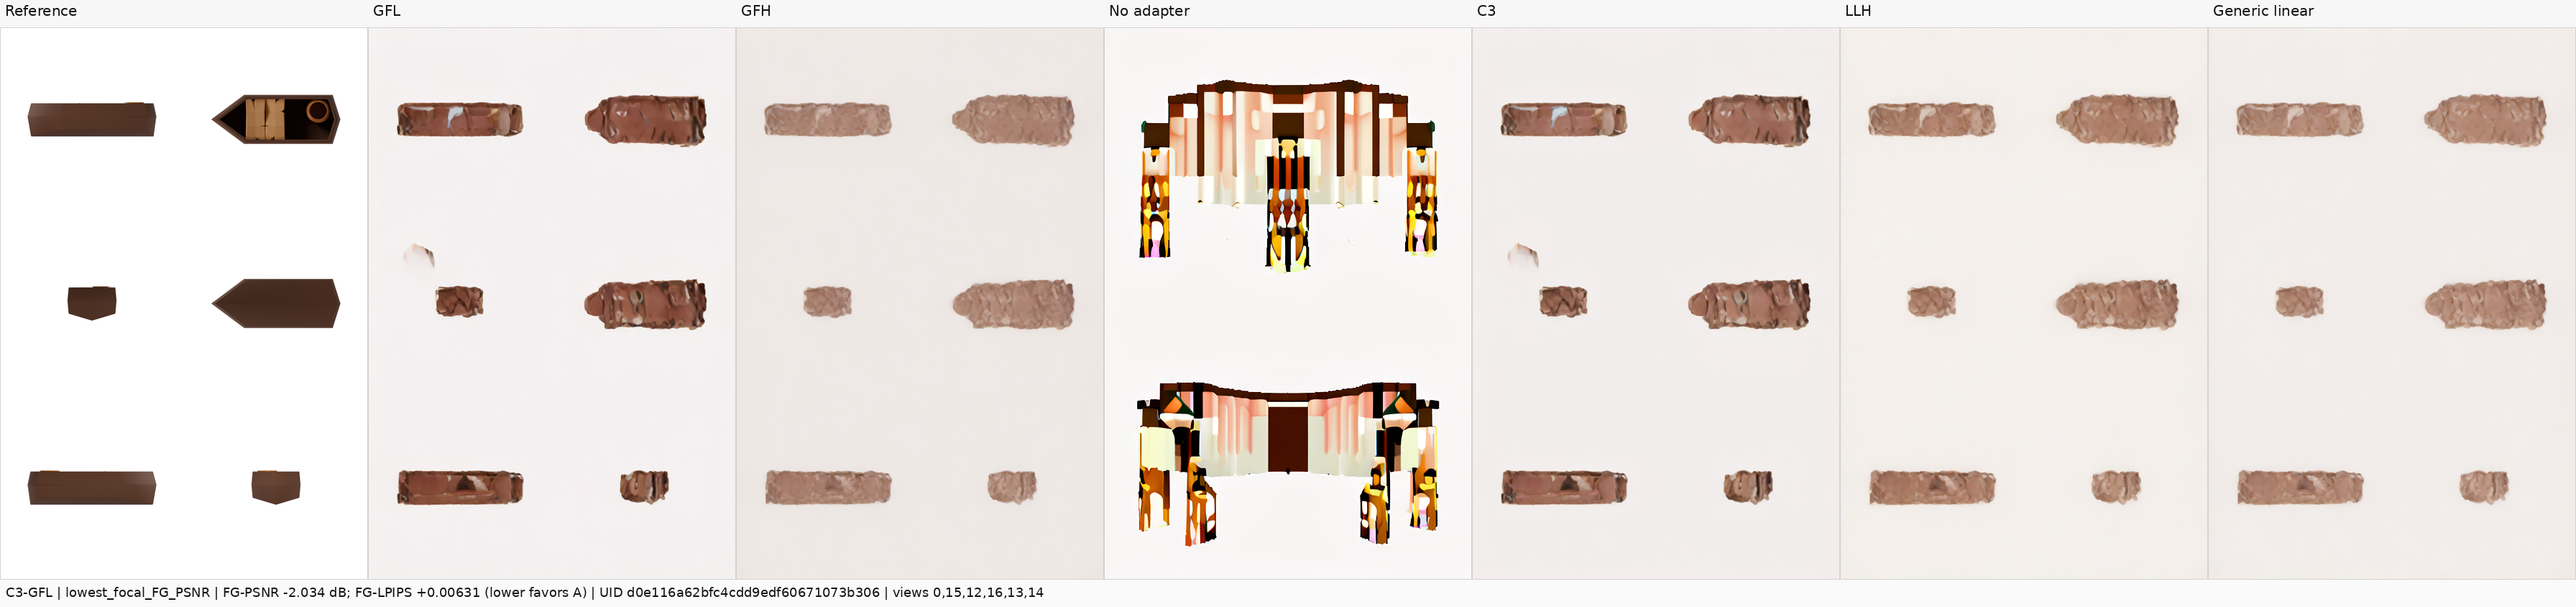
\includegraphics[width=\textwidth,trim=0 36pt 0 0,clip]{figures/figS1_adverse_c3_gfl.png}
\caption{Selected illustrative adverse C3--GFL case from the rights-cleared Fresh C 2D pool. It is not a representative estimate and does not support color-correction, PBR, seam, or human-preference claims.}
\label{fig:supp-failures}
\end{figure}

The attempted Fresh C 24-object GLB bake did not pass its input/output gate: 9/24 sources had out-of-range native UVs, and 5 assets / 27 primitives used unsupported BLEND. No valid Fresh C 24-object bake results were generated. The seam endpoint is retired because the required seam truth set and native full-panel validation did not pass. No full PBR comparison is available. These checks are limitations, not evidence of method failure or success.

\section*{S8. Statistical authority and reproduction map}
Each numerical result in this Supplement is mapped to the internal claim ledger and scoped result sources. Fresh C primary contrasts use object-level deltas and a locked analysis; requested/applied-scale records use the per-step accounting table. Layer/window and Fresh B results are maintained in separate source summaries, with Fresh B classified as retrospective sensitivity because its lock chronology cannot be authenticated from preserved Git history. The texture-complexity cohort and the color-diagnostic set are separate from Fresh C and from each other. The historical N=20 GLB-native summary has a separate analysis record; no N=20 image assets are redistributed. Original Table 9 and Table 3 below are reproduced only as historical source text with explicit provenance limits; neither is treated as a newly verified current result.

\paragraph{Fresh C identity details.} The 300-object Fresh C list is disjoint by UID from the original eval300, including the 24-object development probe, the 1,118-object training list, and the clean-v2 eval300. The primary four-condition run and same-cohort Generic Linear/LLH addendum use the same frozen checkpoint SHA-256 \texttt{0618d6b2\allowbreak{}84ab47aa\allowbreak{}16d7a89d\allowbreak{}c447f5ba\allowbreak{}4455ff6c\allowbreak{}9d918e5e\allowbreak{}129478a9\allowbreak{}9e0114c0}, runner source SHA-256 \texttt{e5c28e915ba137d3541eb4c032daaf62a798332d63b32917b749fe1bcc74e9e3}, cohort, input tensors, endpoint implementation, and seed policy. The seed is $42+\texttt{object\_idx}$ and is shared across the matched conditions for each object. Primary and addendum integrity gates pass for 1,200/1,200 and 600/600 condition rows. Fresh C uses the recorded deep/middle/shallow caps of 3.0/3.5/0.8, with requested, applied, and residual scales logged separately. This is a held-out paired comparison under the stated protocol. The historical identity remains explicit: 01549 names v1 weights for its main tables and a separate v2 strong-residual, per-layer-capped instance for Section 4.7/FAC. Fresh C uses a controlled retraining and is not presented as a numerical reproduction of the old Table 4 $+0.96$ dB estimate.
\section*{S9. Historical 01549 Table 9: strict-276 schedule transfer}

The 01549 submission reports this schedule-transfer comparison on the 276 objects disjoint from the 24-object probe. It uses the strong-residual, per-layer-capped v2 adapter, not the v1 checkpoint named for 01549 Table 4. The values below are reproduced from the authenticated 01549 submission; they are not pooled with Fresh C or the separate MAIN-STAGE-276 profile-placement analysis. The table therefore documents schedule transfer on its stated adapter instance and remains distinct from Fresh C's matched single-checkpoint comparison.

\begin{table}[ht]
\centering\small
\caption{Values reproduced from original 01549 Table 9 for the stated strict-276 retrospective schedule-transfer comparison. The adapter/run differs from Fresh C; row-level runner and input provenance are incomplete. Values are preserved as submitted historical results, not independently verified statistics.}
\label{tab:historical-table9}
\begin{tabular}{lcccc}
\toprule
Schedule & FG-SSIM & PSNR & C3--schedule $\Delta$PSNR (95\% CI) & C3-favourable objects \\
\midrule
Trapezoid & 0.356 & 19.04 & $+0.258$ $[+0.207,+0.308]$ & 206/276 \\
Gaussian peak & 0.358 & 18.97 & $+0.324$ $[+0.281,+0.367]$ & 232/276 \\
Linear warm-up & 0.377 & 18.97 & $+0.323$ $[+0.263,+0.386]$ & 214/276 \\
Cosine bump & 0.330 & 18.39 & $+0.902$ $[+0.824,+0.981]$ & 253/276 \\
C3 (TCAS) & 0.376 & 19.29 & -- & -- \\
\bottomrule
\end{tabular}
\end{table}

\section*{S10. Historical 01549 Table 3: extended 24-object development diagnostics}

The table below is transcribed from the authenticated 01549 source and moved from the main text to preserve the original 24-object development record. The candidate-level row outputs and selection-time provenance are unavailable for independent reanalysis. Laplacian variance, RGB standard deviation, gradient magnitude, and high-frequency energy are variation diagnostics; this historical table does not establish texture fidelity, a population effect, or an optimal schedule.

\begin{table}[ht]
\centering\small
\caption{Values transcribed from original 01549 Table 3 for representative variants in the 24-object development probe. These are historical values, not independently recomputed statistics; variation measures do not establish texture fidelity.}\label{tab:historical-table3}
\begin{tabular}{lcccc}
\toprule
Variant & $\Delta$Lap Var & $\Delta$RGB Std & $\Delta$Grad & $\Delta$HF Energy \\
\midrule
C3 & $-$0.001 & $-$0.023 & +0.142 & +0.058 \\
C4 & $-$0.012 & $-$0.032 & +0.086 & +0.062 \\
A\_s2.50 & $-$0.011 & $-$0.044 & +0.054 & +0.078 \\
A\_s2.00 & $-$0.006 & $-$0.040 & +0.100 & +0.070 \\
A\_s1.25 & $-$0.005 & $-$0.032 & +0.104 & +0.053 \\
\bottomrule
\end{tabular}
\end{table}


\section*{S11. First-round FAC controlled re-examination}
The 01549 first-round package reports seven trained FAC configurations under the paired 300-object protocol. All values below are retained as originally reported; this is not a new 1008 training run. The 12-object untrained C3-envelope control is separate and is described in the main text.

\begin{longtable}{p{3.3cm}p{3.5cm}rrrr}
\caption{FAC dose-response table reported in the first-round 01549 supplement. FG-PSNR and FG-SSIM are the reported absolute values; $\Delta$FG-PSNR and wins compare each trained configuration with TCAS.}\label{tab:fac-dose-response}\\
\toprule
Configuration & Temporal gate & FG-PSNR & FG-SSIM & $\Delta$FG-PSNR & Wins \\
\midrule\endfirsthead
\toprule
Configuration & Temporal gate & FG-PSNR & FG-SSIM & $\Delta$FG-PSNR & Wins \\
\midrule\endhead
TCAS baseline (C3) & fixed C3 & 9.88 & 0.3681 & -- & -- \\
LTAG only & joint, unconstrained & 7.79 & 0.3487 & $-2.08$ & 4/300 \\
LTAG+GSG & joint, unconstrained & 7.03 & 0.3163 & $-2.84$ & 6/300 \\
Full FAC & joint, unconstrained & 6.94 & 0.3204 & $-2.94$ & 5/300 \\
Two-stage + GSG/FSC & frozen at C3 & 7.32 & 0.3074 & $-2.56$ & 4/300 \\
Envelope penalty ($\lambda=1$) & joint, penalized to C3 & 7.14 & 0.3021 & $-2.74$ & 2/300 \\
Fidelity weighting & frozen at C3 & 7.51 & 0.3110 & $-2.37$ & 5/300 \\
Gentle schedule & frozen at C3 & 8.77 & 0.4175 & $-1.10$ & 48/300 \\
\bottomrule
\end{longtable}

The submitted protocol states that only the LTAG/GSG/FSC controllers (roughly $6\times10^3$ parameters) were trained; the base model, VAE, and GeoTex-Adapter remained frozen. It specifies the enhanced latent denoising objective and 2,000 AdamW steps on a training pool stated as 1,706 objects. The separate 12-object untrained control was reported at $\Delta$FG-PSNR $=-0.18$ dB (95\% CI [$-0.42,+0.05$]). A recovered configuration instead lists 1,200 training objects, and no run-bound seed/output manifest was found. We retain the original values as reported, disclose this reproducibility limit, and make no code-release claim.

\section*{S12. Retrospective texture-complexity boundary}
This analysis uses the separate FRESH\_CONFIRM\_300 cohort ($N=300$), not Fresh C or Fresh B. LLH and native GFL rows match the frozen object list and share the recorded checkpoint, runner, seed, six unique target views, sampler, and protocol. The paired LLH--GFL mean differences are $+1.2877$ dB FG-PSNR (95\% object-bootstrap CI [$+0.9383,+1.6346$]; 57.7\% LLH-favorable objects) and $-0.01650$ FG-LPIPS ([$-0.01887,-0.01413$]; 73.3\% LLH-favorable objects).

The descriptor analysis tests two image-space outcomes against five ground-truth descriptors: foreground Laplacian variance, RGB standard deviation, gradient magnitude, high-frequency energy, and coverage. Spearman correlations use average ranks and paired-object percentile bootstrap intervals (10,000 resamples, seed 20261002). The family contains ten plus-one-corrected bootstrap sign tests and Holm correction across all ten. Nine tests reject at 0.05; the only non-rejection is FG-LPIPS versus coverage (adjusted $p=0.0508$). The preserved H5 hypothesis excerpt predates one archived outcome bundle, but the main multiplicity lock classifies this family as retrospective after prior outcome exposure; that chronology has not been reconciled. We therefore report all associations as retrospective sensitivity evidence, not as preregistered confirmation.

\begin{table}[ht]
\centering\scriptsize
\caption{Retrospective Spearman associations between LLH--GFL image-space deltas and ground-truth descriptors in FRESH\_CONFIRM\_300. Correlation intervals are paired-object bootstrap intervals; adjusted $p$ values use the ten-test Holm family with plus-one-corrected bootstrap sign tests.}
\label{tab:texture-complexity}
\begin{tabular}{llrrl}
\toprule Outcome delta & Ground-truth descriptor & $\rho$ [95\% CI] & Holm $p$ & Decision \\
\midrule
FG-PSNR & Laplacian variance & $-0.524$ [$-0.603,-0.435$] & 0.0020 & reject \\
FG-PSNR & RGB standard deviation & $-0.380$ [$-0.488,-0.266$] & 0.0020 & reject \\
FG-PSNR & Gradient magnitude & $-0.464$ [$-0.548,-0.371$] & 0.0020 & reject \\
FG-PSNR & High-frequency energy & $-0.691$ [$-0.745,-0.626$] & 0.0020 & reject \\
FG-PSNR & Foreground coverage & $-0.134$ [$-0.241,-0.026$] & 0.0352 & reject \\
FG-LPIPS & Laplacian variance & $+0.604$ [$+0.511,+0.681$] & 0.0020 & reject \\
FG-LPIPS & RGB standard deviation & $+0.379$ [$+0.272,+0.482$] & 0.0020 & reject \\
FG-LPIPS & Gradient magnitude & $+0.563$ [$+0.469,+0.643$] & 0.0020 & reject \\
FG-LPIPS & High-frequency energy & $+0.677$ [$+0.599,+0.744$] & 0.0020 & reject \\
FG-LPIPS & Foreground coverage & $-0.118$ [$-0.233,+0.0002$] & 0.0508 & not rejected \\
\bottomrule
\end{tabular}
\end{table}

Ground-truth foreground Laplacian-variance quartiles contain 75 objects each. The FG-PSNR mean LLH--GFL difference declines from $+4.140$ dB in Q1 (92.0\% favor LLH) to $+1.127$ dB in Q2 (52.0\%), $-0.087$ dB in Q3 (41.3\%), and $-0.029$ dB in Q4 (45.3\%). The FG-LPIPS mean changes are $-0.03745$, $-0.01665$, $-0.00670$, and $-0.00520$ from Q1 to Q4; the favorable-object rates decline from 97.3\% to 50.7\%. These strata describe heterogeneity in this cohort. They do not establish that texture complexity causes the response, define a threshold, validate an object selector, or measure texture fidelity.

\clearpage
\section*{S13. Paired color-pathway diagnosis and failure boundaries}
The color diagnosis is a selected, failure-enriched set of six earlier cases and 20 Fresh C panels; it is neither random nor a new holdout. No Adapter, GFL, and LLH were compared on the same inputs, checkpoint, and runner across six unique target views (78 object-condition records). CIEDE2000 was recomputed from hash-identified RGB and frozen masks. Intervals are descriptive paired object bootstraps (20,000 resamples, seed 61008); no confirmatory multiplicity family was defined. Figure~6 shows one of the 20 Fresh C panels (UID \texttt{f6979d7ff8e54c4daf00fee46f09a139}); its pre-existing C3--GFL stratum was lowest FG-LPIPS, not color-based, and it is distinct from the legacy pink-shift cases.

\begin{table}[ht]
\centering\scriptsize
\caption{Selected paired endpoints from the failure-enriched 26-object color diagnosis. Each row is condition A minus B with an object-level 95\% paired-bootstrap CI. Lower CIEDE2000 and FG-LPIPS are favorable; higher PSNR and Edge-SSIM are favorable. Local texture statistics describe variation, not fidelity.}
\label{tab:color-diagnostic}
\begin{tabular}{llrr}
\toprule Contrast & Endpoint & Mean difference & 95\% CI \\
\midrule
GFL -- No Adapter & Foreground CIEDE2000 & $-19.654$ & [$-26.370,-13.248$] \\
GFL -- No Adapter & FG-PSNR (dB) & $+6.646$ & [$+5.556,+7.635$] \\
GFL -- No Adapter & FG-LPIPS & $-0.03251$ & [$-0.05363,-0.01072$] \\
GFL -- No Adapter & Edge-SSIM & $+0.06510$ & [$+0.04853,+0.08202$] \\
LLH -- GFL & Foreground CIEDE2000 & $+3.583$ & [$+0.462,+6.712$] \\
LLH -- GFL & FG-PSNR (dB) & $-0.197$ & [$-1.562,+1.297$] \\
LLH -- GFL & FG-LPIPS & $-0.01294$ & [$-0.02742,+0.00066$] \\
LLH -- GFL & Edge-SSIM & $-0.00080$ & [$-0.00776,+0.00659$] \\
LLH -- GFL & Foreground gradient magnitude & $-0.06772$ & [$-0.08132,-0.05494$] \\
LLH -- GFL & Foreground high-frequency energy & $-0.00887$ & [$-0.01091,-0.00672$] \\
LLH -- GFL & Foreground color entropy & $-0.598$ & [$-0.703,-0.502$] \\
\bottomrule
\end{tabular}
\end{table}

GFL lowered reference-relative CIEDE2000 in 24/26 objects, but visible pink or purple remained in two legacy cases under all three conditions. LLH increased mean color error while reducing local variation, not fidelity. The RGB shift was visible before baking and at denoising update 40. For one case, a ground-truth VAE round trip gave CIEDE2000 4.086 and $\Delta a^*\approx-1.35$, versus 22.032 and $+1.977$ for GFL; this weakens a VAE-only explanation but does not identify the cause.

A locked P0 trace of three preselected objects reproduced saved RGB pixels exactly in repeated Python 3.13.5 runs; Python 3.10 reproduced its corresponding archived observer. The first cross-runtime tensor difference followed multiplication of the shared FP16 initial latent by the scheduler noise scale (maximum absolute difference 0.0625; RMSE 0.00966; 32.3\% changed). This resolves output identity only for these three traces; it establishes neither cohort-wide cross-stack equivalence nor the color cause.

The feature-relative residual gate increased mean CIEDE2000 by 1.35 across 26 objects and 3.18 in the six earlier cases, with no clear visual improvement. The complete cause remains unresolved; no repair is validated.

\section*{S16. Matched applied-budget comparison and revision validity corrections}
The same-cohort GeoTex addendum contains 300 objects by six conditions, 1,800 rows. Each object uses the same initial latent, input tensors and checkpoint across conditions. Early-, Middle- and Late-high use 16 high updates at 0--15, 17--32 and 34--49. Low/high are 1.25/2.50, Fixed Mean is 1.65, and the native shallow cap is 0.8. Their exact applied per-group sums are 82.5, 82.5 and 40. This comparison measures the total effect of allocating the high segment at equal applied scalar budget. Evolving residual norms are outcomes of the trajectory; lack of equal residual norms limits a mechanism interpretation, not validity of the allocation contrast. The study is post-inspection on the already evaluated Fresh C objects, not an independent confirmation.

\begingroup\scriptsize
\begin{longtable}{llll}
\caption{Selected paired contrasts from the 300-object equal-budget addendum. Mean A minus B and pointwise 95\% object-bootstrap interval (50,000 resamples). The other 59 pair--metric contrasts form one post hoc Holm family; no interval is multiplicity-adjusted.}\label{tab:budget300paired}\\
\toprule Contrast & Endpoint & Mean [95\% CI] & Holm $p$ \\
\midrule\endfirsthead
\toprule Contrast & Endpoint & Mean [95\% CI] & Holm $p$ \\
\midrule\endhead
Middle $-$ Fixed Applied Mean & fg-psnr & $-0.13326\ [-0.16979,-0.09622]$ & 1e-05 (raw) \\
Middle $-$ Fixed Applied Mean & fg-lpips & $+0.00199\ [+0.00147,+0.00254]$ & 0.00059 \\
Middle $-$ Fixed Applied Mean & fg-ssim & $-0.01185\ [-0.01347,-0.01025]$ & 0.00059 \\
Middle $-$ Fixed Applied Mean & edge-ssim & $-0.00703\ [-0.00764,-0.00643]$ & 0.00059 \\
Middle $-$ Late-high & fg-psnr & $-0.56395\ [-0.63408,-0.49427]$ & 0.00059 \\
Middle $-$ Late-high & fg-lpips & $+0.00466\ [+0.00381,+0.00553]$ & 0.00059 \\
Middle $-$ Late-high & fg-ssim & $-0.00422\ [-0.00694,-0.00139]$ & 0.01375 \\
Middle $-$ Late-high & edge-ssim & $-0.01409\ [-0.01526,-0.01291]$ & 0.00059 \\
Middle $-$ Early-high & fg-psnr & $+0.49619\ [+0.37195,+0.62282]$ & 0.00059 \\
Middle $-$ Early-high & fg-lpips & $-0.00472\ [-0.00568,-0.00378]$ & 0.00059 \\
Middle $-$ Early-high & fg-ssim & $+0.00499\ [+0.00211,+0.00809]$ & 0.00432 \\
Middle $-$ Early-high & edge-ssim & $+0.00080\ [-0.00008,+0.00170]$ & 0.1565 \\
Middle $-$ Fixed High & fg-psnr & $-0.74767\ [-0.88995,-0.60691]$ & 0.00059 \\
Middle $-$ Fixed High & fg-lpips & $+0.01070\ [+0.00889,+0.01255]$ & 0.00059 \\
Middle $-$ Fixed High & fg-ssim & $-0.04553\ [-0.04937,-0.04165]$ & 0.00059 \\
Middle $-$ Fixed High & edge-ssim & $-0.01881\ [-0.02083,-0.01678]$ & 0.00059 \\
\bottomrule
\end{longtable}\endgroup
The named Middle--Fixed Mean FG-PSNR endpoint is shown with its raw $p$; remaining 59 contrasts use a common post hoc Holm correction in the delivered recomputation. All are retrospective. The rank counts in main matched-budget table are not cross-metric superiority tests.

\paragraph{Validity corrections to earlier native experiments.}
The earlier seven-object MV-Adapter temporal archive passed source-path identity, but used Fresh C targets with a different mesh normalization and orthographic range. In an input-only native geometry audit, one object's six foreground IoUs were about 0.21--0.61. Its old quality estimates are therefore not validated native-camera cross-backbone evidence; the original identity test remains valid. The new targets use the exact native mesh loader, orthographic cameras and nvdiffrast rasterizer, with a source embedded base-color texture and white background. This is unlit albedo, not a claim of PBR or source-render lighting equivalence.

The earlier five-object bake rotated generated pole-view RGB back into raw-camera coordinates but also incorrectly rotated the raw-camera mask. Four of five objects have affected masks. Its old quality estimates are superseded by corrected evaluation and are not pooled with newly selected objects. In the REPEAT branch, bilinear fractions must be calculated before wrapping integer indices: the previous order could produce negative weights at tile edges and outside [0,1]. Corrected code passes nonnegative/unit-sum weight checks and integer-period translation invariance. Scalar coverage masks are read without an RGB transfer function; decoding grayscale coverage as sRGB would change the foreground threshold. GT source images are resized to 256 using bicubic RGB and the same nearest-index alpha masks as generated sources; atlas, camera, fill and render parameters are shared. The original GT-512 bake is retained only as an unmatched-resolution diagnostic.

\paragraph{Default-path identity boundary.}
For GeoTex, explicit requested scale 1.0 and an unset scale are different: the cap is applied only when the scale attribute exists. Executing the actual wrapper with a unit residual gives deep/middle/shallow applied factors (1,1,0.8) for explicit 1.0, versus (1,1,1) when unset. The stored condition name \texttt{native\_default\_1x} therefore denotes Constant 1.0 (capped), not an unmodified pipeline. This is a wrapper-level counterexample, not a claim of full-pipeline pixel equality. In contrast, the new MV-Adapter identity gate compares three textured meshes and 18 images: official default, deployed default and a constant-1 schedule produce bitwise-identical RGB pixels, condition-encoder features and injected residuals. The 13 texture-absent MV-Adapter inputs use the documented geometry-only loader compatibility branch; their targets are constant white albedo and remain in the primary cohort.



\clearpage
\section*{S17. Frozen native MV-Adapter comparison on fifty new-to-interface objects}
The protocol was internally frozen before new scheduled outputs; it is not a public preregistration. Fifty inputs were selected in UID order from Fresh C after excluding every recorded previously inspected MV-Adapter UID. Selection uses available inputs and native geometry/material criteria, not quality or parameter search. Seeds are $20261010+\mathrm{index}$, shared across conditions. Six native-camera 512-pixel images use 50 DDPM-shift updates, CFG 3, reference strength 1 and the frozen high-quality text prompt. All 350 rows completed. Models, input identities, runner, native-target calibration and per-step residual traces are indexed in the reproduction archive.

Early-, Middle- and Late-high use high=1 over steps 0--15, 17--32 and 34--49 respectively, with low=0.75 elsewhere. Fixed Mean=0.83 and Generic Linear spans 0.75--0.91 inclusively; each sums to 41.5 per feature, whereas Native/Fixed High sums to 50 and Fixed Low to 37.5. These are feature-scaling controls on MV-Adapter, not GeoTex's per-ResNet capped residual doses.

Official/deployed default and constant-1 scheduled paths match exactly on three textured new objects, including 18 RGB images, encoded conditions and injected residuals. Native target geometry positions/masks match the control rasterization for all fifty inputs; an independent CPU bilinear source-UV sample agrees within the frozen tolerance. Thirteen texture-absent assets use geometry-only compatibility loading and white target albedo; they remain in the primary fifty. The 37-object textured subset is descriptive. It does not create a second primary or substitute after observing outcomes.

The primary Middle-high--Fixed Mean FG-PSNR mean is $+0.02899$ dB, 95\% CI $[-0.01941,+0.08074]$, Monte Carlo sign-flip $p=0.28075$ (100,000 draws, plus-one correction); 29/50 favor Middle. Intervals use 50,000 object resamples. The other 104 contrasts (21 condition pairs by five endpoints, minus primary) form one predeclared Holm family; intervals remain pointwise. No non-inferiority or architecture-causal claim follows from a non-separated contrast.

\begingroup\scriptsize
\begin{longtable}{llrr}
\caption{Complete native fifty-object pair--metric contrasts. A minus B; lower LPIPS/CIEDE2000 and higher other endpoints are favorable. $p$ is Holm-adjusted except the single primary marked raw.}\label{tab:mva50-paired}\\
\toprule A -- B & Endpoint & Mean [95\% CI] & $p$ \\
\midrule\endfirsthead
\toprule A -- B & Endpoint & Mean [95\% CI] & $p$ \\
\midrule\endhead
High -- Low & fg-psnr & $-0.12682\ [-0.24503,-0.02980]$ & 0.85601 \\
High -- Low & fg-lpips & $+0.00100\ [-0.00197,+0.00592]$ & 1.00000 \\
High -- Low & fg-ssim & $-0.00250\ [-0.00594,+0.00029]$ & 1.00000 \\
High -- Low & edge-ssim & $+0.00511\ [+0.00114,+0.00979]$ & 0.85601 \\
High -- Low & ciede2000 & $+0.44730\ [+0.13967,+0.87441]$ & 0.20880 \\
High -- Mean & fg-psnr & $-0.08309\ [-0.16282,-0.02065]$ & 0.78170 \\
High -- Mean & fg-lpips & $+0.00013\ [-0.00120,+0.00214]$ & 1.00000 \\
High -- Mean & fg-ssim & $-0.00268\ [-0.00534,-0.00051]$ & 1.00000 \\
High -- Mean & edge-ssim & $+0.00163\ [-0.00023,+0.00339]$ & 1.00000 \\
High -- Mean & ciede2000 & $+0.33298\ [+0.10737,+0.65171]$ & 0.13932 \\
High -- Early & fg-psnr & $+0.00563\ [-0.03952,+0.05131]$ & 1.00000 \\
High -- Early & fg-lpips & $-0.00158\ [-0.00243,-0.00081]$ & 0.01649 \\
High -- Early & fg-ssim & $+0.00002\ [-0.00176,+0.00171]$ & 1.00000 \\
High -- Early & edge-ssim & $+0.00228\ [-0.00040,+0.00477]$ & 1.00000 \\
High -- Early & ciede2000 & $+0.03229\ [-0.06895,+0.13756]$ & 1.00000 \\
High -- Middle & fg-psnr & $-0.11208\ [-0.22257,-0.02534]$ & 0.89608 \\
High -- Middle & fg-lpips & $+0.00175\ [-0.00105,+0.00664]$ & 1.00000 \\
High -- Middle & fg-ssim & $-0.00200\ [-0.00524,+0.00047]$ & 1.00000 \\
High -- Middle & edge-ssim & $+0.00562\ [+0.00250,+0.00961]$ & 0.02112 \\
High -- Middle & ciede2000 & $+0.41481\ [+0.13251,+0.81706]$ & 0.14875 \\
High -- Late & fg-psnr & $-0.14046\ [-0.25619,-0.04753]$ & 0.26910 \\
High -- Late & fg-lpips & $+0.00203\ [-0.00108,+0.00734]$ & 1.00000 \\
High -- Late & fg-ssim & $-0.00341\ [-0.00673,-0.00079]$ & 0.87002 \\
High -- Late & edge-ssim & $+0.00119\ [-0.00198,+0.00545]$ & 1.00000 \\
High -- Late & ciede2000 & $+0.47923\ [+0.17811,+0.90198]$ & 0.05490 \\
High -- Linear & fg-psnr & $-0.12216\ [-0.22718,-0.04049]$ & 0.22752 \\
High -- Linear & fg-lpips & $+0.00174\ [-0.00098,+0.00639]$ & 1.00000 \\
High -- Linear & fg-ssim & $-0.00309\ [-0.00618,-0.00068]$ & 0.90959 \\
High -- Linear & edge-ssim & $+0.00243\ [-0.00040,+0.00605]$ & 1.00000 \\
High -- Linear & ciede2000 & $+0.42004\ [+0.14924,+0.81173]$ & 0.05005 \\
Low -- Mean & fg-psnr & $+0.04373\ [-0.00118,+0.09206]$ & 1.00000 \\
Low -- Mean & fg-lpips & $-0.00087\ [-0.00381,+0.00085]$ & 1.00000 \\
Low -- Mean & fg-ssim & $-0.00017\ [-0.00118,+0.00090]$ & 1.00000 \\
Low -- Mean & edge-ssim & $-0.00348\ [-0.00757,-0.00081]$ & 0.36480 \\
Low -- Mean & ciede2000 & $-0.11432\ [-0.24502,-0.00126]$ & 1.00000 \\
Low -- Early & fg-psnr & $+0.13245\ [+0.04720,+0.24287]$ & 0.15288 \\
Low -- Early & fg-lpips & $-0.00258\ [-0.00777,+0.00036]$ & 1.00000 \\
Low -- Early & fg-ssim & $+0.00253\ [+0.00006,+0.00594]$ & 1.00000 \\
Low -- Early & edge-ssim & $-0.00283\ [-0.00657,-0.00016]$ & 1.00000 \\
Low -- Early & ciede2000 & $-0.41501\ [-0.81018,-0.14622]$ & 0.04876 \\
Low -- Middle & fg-psnr & $+0.01475\ [-0.01731,+0.04840]$ & 1.00000 \\
Low -- Middle & fg-lpips & $+0.00075\ [+0.00030,+0.00122]$ & 0.17384 \\
Low -- Middle & fg-ssim & $+0.00050\ [-0.00056,+0.00160]$ & 1.00000 \\
Low -- Middle & edge-ssim & $+0.00051\ [-0.00072,+0.00181]$ & 1.00000 \\
Low -- Middle & ciede2000 & $-0.03249\ [-0.10291,+0.03715]$ & 1.00000 \\
Low -- Late & fg-psnr & $-0.01363\ [-0.02840,+0.00083]$ & 1.00000 \\
Low -- Late & fg-lpips & $+0.00103\ [+0.00051,+0.00167]$ & 0.00800 \\
Low -- Late & fg-ssim & $-0.00091\ [-0.00156,-0.00021]$ & 0.79142 \\
Low -- Late & edge-ssim & $-0.00392\ [-0.00547,-0.00234]$ & 0.00303 \\
Low -- Late & ciede2000 & $+0.03193\ [+0.00504,+0.05951]$ & 1.00000 \\
Low -- Linear & fg-psnr & $+0.00467\ [-0.02786,+0.03373]$ & 1.00000 \\
Low -- Linear & fg-lpips & $+0.00074\ [+0.00032,+0.00118]$ & 0.09680 \\
Low -- Linear & fg-ssim & $-0.00058\ [-0.00154,+0.00033]$ & 1.00000 \\
Low -- Linear & edge-ssim & $-0.00267\ [-0.00418,-0.00118]$ & 0.10701 \\
Low -- Linear & ciede2000 & $-0.02726\ [-0.09723,+0.04844]$ & 1.00000 \\
Mean -- Early & fg-psnr & $+0.08872\ [+0.03375,+0.16183]$ & 0.07565 \\
Mean -- Early & fg-lpips & $-0.00171\ [-0.00411,-0.00028]$ & 0.42750 \\
Mean -- Early & fg-ssim & $+0.00270\ [+0.00064,+0.00545]$ & 0.78170 \\
Mean -- Early & edge-ssim & $+0.00065\ [-0.00092,+0.00210]$ & 1.00000 \\
Mean -- Early & ciede2000 & $-0.30069\ [-0.59160,-0.11032]$ & 0.02280 \\
Middle -- Mean & fg-psnr & $+0.02899\ [-0.01941,+0.08074]$ & 0.28075 (raw) \\
Mean -- Middle & fg-lpips & $+0.00162\ [-0.00005,+0.00462]$ & 1.00000 \\
Mean -- Middle & fg-ssim & $+0.00067\ [-0.00064,+0.00204]$ & 1.00000 \\
Mean -- Middle & edge-ssim & $+0.00399\ [+0.00170,+0.00764]$ & 0.00104 \\
Mean -- Middle & ciede2000 & $+0.08184\ [-0.02823,+0.20315]$ & 1.00000 \\
Mean -- Late & fg-psnr & $-0.05737\ [-0.10476,-0.01422]$ & 0.85601 \\
Mean -- Late & fg-lpips & $+0.00190\ [-0.00003,+0.00530]$ & 1.00000 \\
Mean -- Late & fg-ssim & $-0.00074\ [-0.00183,+0.00031]$ & 1.00000 \\
Mean -- Late & edge-ssim & $-0.00044\ [-0.00301,+0.00363]$ & 1.00000 \\
Mean -- Late & ciede2000 & $+0.14625\ [+0.03581,+0.27574]$ & 0.87002 \\
Mean -- Linear & fg-psnr & $-0.03907\ [-0.07392,-0.01081]$ & 0.57941 \\
Mean -- Linear & fg-lpips & $+0.00161\ [+0.00009,+0.00434]$ & 1.00000 \\
Mean -- Linear & fg-ssim & $-0.00041\ [-0.00129,+0.00045]$ & 1.00000 \\
Mean -- Linear & edge-ssim & $+0.00081\ [-0.00123,+0.00410]$ & 1.00000 \\
Mean -- Linear & ciede2000 & $+0.08707\ [+0.01651,+0.17259]$ & 1.00000 \\
Early -- Middle & fg-psnr & $-0.11771\ [-0.23017,-0.02649]$ & 0.98234 \\
Early -- Middle & fg-lpips & $+0.00333\ [+0.00036,+0.00863]$ & 0.57941 \\
Early -- Middle & fg-ssim & $-0.00203\ [-0.00568,+0.00081]$ & 1.00000 \\
Early -- Middle & edge-ssim & $+0.00334\ [+0.00057,+0.00690]$ & 1.00000 \\
Early -- Middle & ciede2000 & $+0.38253\ [+0.11622,+0.76613]$ & 0.19845 \\
Early -- Late & fg-psnr & $-0.14609\ [-0.25687,-0.06083]$ & 0.03572 \\
Early -- Late & fg-lpips & $+0.00361\ [+0.00036,+0.00933]$ & 0.80715 \\
Early -- Late & fg-ssim & $-0.00344\ [-0.00694,-0.00080]$ & 0.80715 \\
Early -- Late & edge-ssim & $-0.00109\ [-0.00429,+0.00294]$ & 1.00000 \\
Early -- Late & ciede2000 & $+0.44694\ [+0.17823,+0.84174]$ & 0.01089 \\
Early -- Linear & fg-psnr & $-0.12778\ [-0.22984,-0.04995]$ & 0.03572 \\
Early -- Linear & fg-lpips & $+0.00332\ [+0.00045,+0.00838]$ & 0.31416 \\
Early -- Linear & fg-ssim & $-0.00311\ [-0.00648,-0.00061]$ & 1.00000 \\
Early -- Linear & edge-ssim & $+0.00016\ [-0.00259,+0.00353]$ & 1.00000 \\
Early -- Linear & ciede2000 & $+0.38776\ [+0.14561,+0.75366]$ & 0.01176 \\
Middle -- Late & fg-psnr & $-0.02838\ [-0.05857,-0.00004]$ & 1.00000 \\
Middle -- Late & fg-lpips & $+0.00028\ [-0.00018,+0.00080]$ & 1.00000 \\
Middle -- Late & fg-ssim & $-0.00141\ [-0.00243,-0.00042]$ & 0.66671 \\
Middle -- Late & edge-ssim & $-0.00443\ [-0.00568,-0.00316]$ & 0.00104 \\
Middle -- Late & ciede2000 & $+0.06442\ [-0.00064,+0.12764]$ & 1.00000 \\
Middle -- Linear & fg-psnr & $-0.01008\ [-0.04413,+0.02065]$ & 1.00000 \\
Middle -- Linear & fg-lpips & $-0.00001\ [-0.00041,+0.00033]$ & 1.00000 \\
Middle -- Linear & fg-ssim & $-0.00109\ [-0.00220,-0.00019]$ & 1.00000 \\
Middle -- Linear & edge-ssim & $-0.00318\ [-0.00412,-0.00227]$ & 0.00104 \\
Middle -- Linear & ciede2000 & $+0.00523\ [-0.07199,+0.08600]$ & 1.00000 \\
Late -- Linear & fg-psnr & $+0.01830\ [-0.01050,+0.04259]$ & 1.00000 \\
Late -- Linear & fg-lpips & $-0.00029\ [-0.00101,+0.00020]$ & 1.00000 \\
Late -- Linear & fg-ssim & $+0.00033\ [-0.00046,+0.00100]$ & 1.00000 \\
Late -- Linear & edge-ssim & $+0.00125\ [+0.00038,+0.00194]$ & 0.15288 \\
Late -- Linear & ciede2000 & $-0.05919\ [-0.12493,+0.00991]$ & 1.00000 \\
\bottomrule\end{longtable}\endgroup
\begin{table}[ht]\centering\scriptsize
\caption{Descriptive 37-object textured subset, retained separately from the primary fifty. No subset inference is promoted to confirmation.}
\begin{tabular}{lrrrrr}\toprule Condition & PSNR & LPIPS & SSIM & Edge-SSIM & CIEDE2000 \\
\midrule
High & 14.06 & 0.1159 & 0.4354 & 0.3239 & 18.04 \\
Low & 14.14 & 0.1170 & 0.4345 & 0.3174 & 17.82 \\
Mean & 14.11 & 0.1165 & 0.4356 & 0.3204 & 17.87 \\
Early & 14.06 & 0.1168 & 0.4345 & 0.3182 & 17.99 \\
Middle & 14.12 & 0.1165 & 0.4347 & 0.3182 & 17.84 \\
Late & 14.16 & 0.1164 & 0.4359 & 0.3233 & 17.79 \\
Linear & 14.14 & 0.1164 & 0.4360 & 0.3217 & 17.82 \\
\bottomrule\end{tabular}\end{table}

\clearpage
\section*{S18. Calibrated bake pilot, historical separation and actual-output displays}
The new bake list contains ten objects, chosen in frozen UID order before observing their bake results. All 300 Fresh C inputs were screened; old five-object outputs and the previously inspected REPEAT diagnostic object were excluded. Eligibility required available source GLB, one opaque white-factor base-color material, native TEXCOORD\_0, no vertex colors, at most 300,000 triangles, and source camera-mask alignment passing the frozen gate. This input-selected set is smaller than the target twenty and below fifteen; we retain the pilot designation and all ten outcomes. No failed or adverse-quality object was replaced. Seven conditions generated 70 object-condition rows; eight bake conditions including GT generated 80 artifacts, with 880 unseen renders and 480 source-camera renders.

The frozen primary was Late-high--Fixed Mean FG-LPIPS. C3--GFH PSNR, LPIPS, SSIM and CIEDE2000 form one four-test secondary Holm family. All other complete pairs are descriptive. Views are averaged before inference. Intervals use 50,000 paired object resamples and are pointwise, not simultaneous. The ten-object primary uses all $2^{10}$ sign flips; the secondary family uses the same exact test. A sign-flip test assumes symmetry/exchangeability of paired differences under its null; an interval alone is not a practical-equivalence criterion. No non-inferiority margin was chosen.

\begin{table}[ht]\centering\scriptsize
\caption{Prespecified new-pilot comparisons: raw A minus B, 95\% object-bootstrap interval; no pooling with old five.}\label{tab:bake-paired}
\begin{tabular}{llrr}
\toprule Contrast & Endpoint & Mean [95\% CI] & $p$ \\
\midrule
Late--Mean & FG-LPIPS & $-0.00265\ [-0.00414,-0.00137]$ & 0.00195 (primary) \\
C3--GFH & FG-PSNR & $+0.193\ [-0.649,+0.875]$ & 1.000 (Holm) \\
C3--GFH & FG-LPIPS & $-0.00036\ [-0.00396,+0.00336]$ & 1.000 (Holm) \\
C3--GFH & FG-SSIM & $-0.05274\ [-0.07459,-0.03170]$ & 0.00781 (Holm) \\
C3--GFH & CIEDE2000 & $-1.102\ [-2.915,+0.939]$ & 0.95508 (Holm) \\
\bottomrule\end{tabular}\end{table}

The corrected earlier five-object bake uses the same source-resolution and mask corrections but retains its historical clamped-UV technical scope. Its descriptive means (PSNR / LPIPS / SSIM) are GFH 11.86 / 0.1609 / 0.5513, C3 14.24 / 0.1542 / 0.4170, Fixed Mean 14.19 / 0.1538 / 0.4348 and Late-high 15.02 / 0.1479 / 0.4428. C3--GFH is $+2.37$ dB, not the superseded $+2.27$ dB estimate. There was no independent predeclared primary for this reevaluation. The older N=20 result, old five, new ten and corrected single-object REPEAT diagnostic each retain separate source identifiers. Earlier wrong-mask, gamma-decoded-alpha and wrong-REPEAT-weight artifacts remain audit records and are superseded, never combined with the valid reevaluation.

\begin{table}[ht]\centering\scriptsize
\caption{Per-object generated-view versus unseen-bake rankings across seven conditions. Bootstrap unit is object. Positive overall agreement does not require an identical winning condition.}
\begin{tabular}{lrr}
\toprule Endpoint & Mean Spearman $\rho$ [95\% CI] & Winner changed \\
\midrule
FG-PSNR & $0.846\ [0.696,0.968]$ & 1/10 \\
FG-LPIPS & $0.804\ [0.693,0.911]$ & 7/10 \\
FG-SSIM & $0.746\ [0.450,0.964]$ & 4/10 \\
Edge-SSIM & $0.907\ [0.871,0.943]$ & 6/10 \\
\bottomrule\end{tabular}\end{table}

GT and generated bake sources use the same six raw cameras and 256-pixel resolution. GT RGB uses bicubic downsampling; alpha uses the exact nearest-index mapping used for generated foreground inputs. Their six-view scalar masks are bitwise identical and their raw atlas coverage matches for every object and condition. No unseen view enters baking. Export checks retain binary geometry/UV buffers, transforms and mesh identity. REPEAT UV weights are nonnegative, sum to one and are invariant under integer UV shifts. These checks establish a valid unlit projection comparison, not PBR equivalence or a validated seam score. Texture boundaries can be natural appearance boundaries; seam diagnostics are not reported as a validated primary endpoint.

\begin{figure}[p]\centering
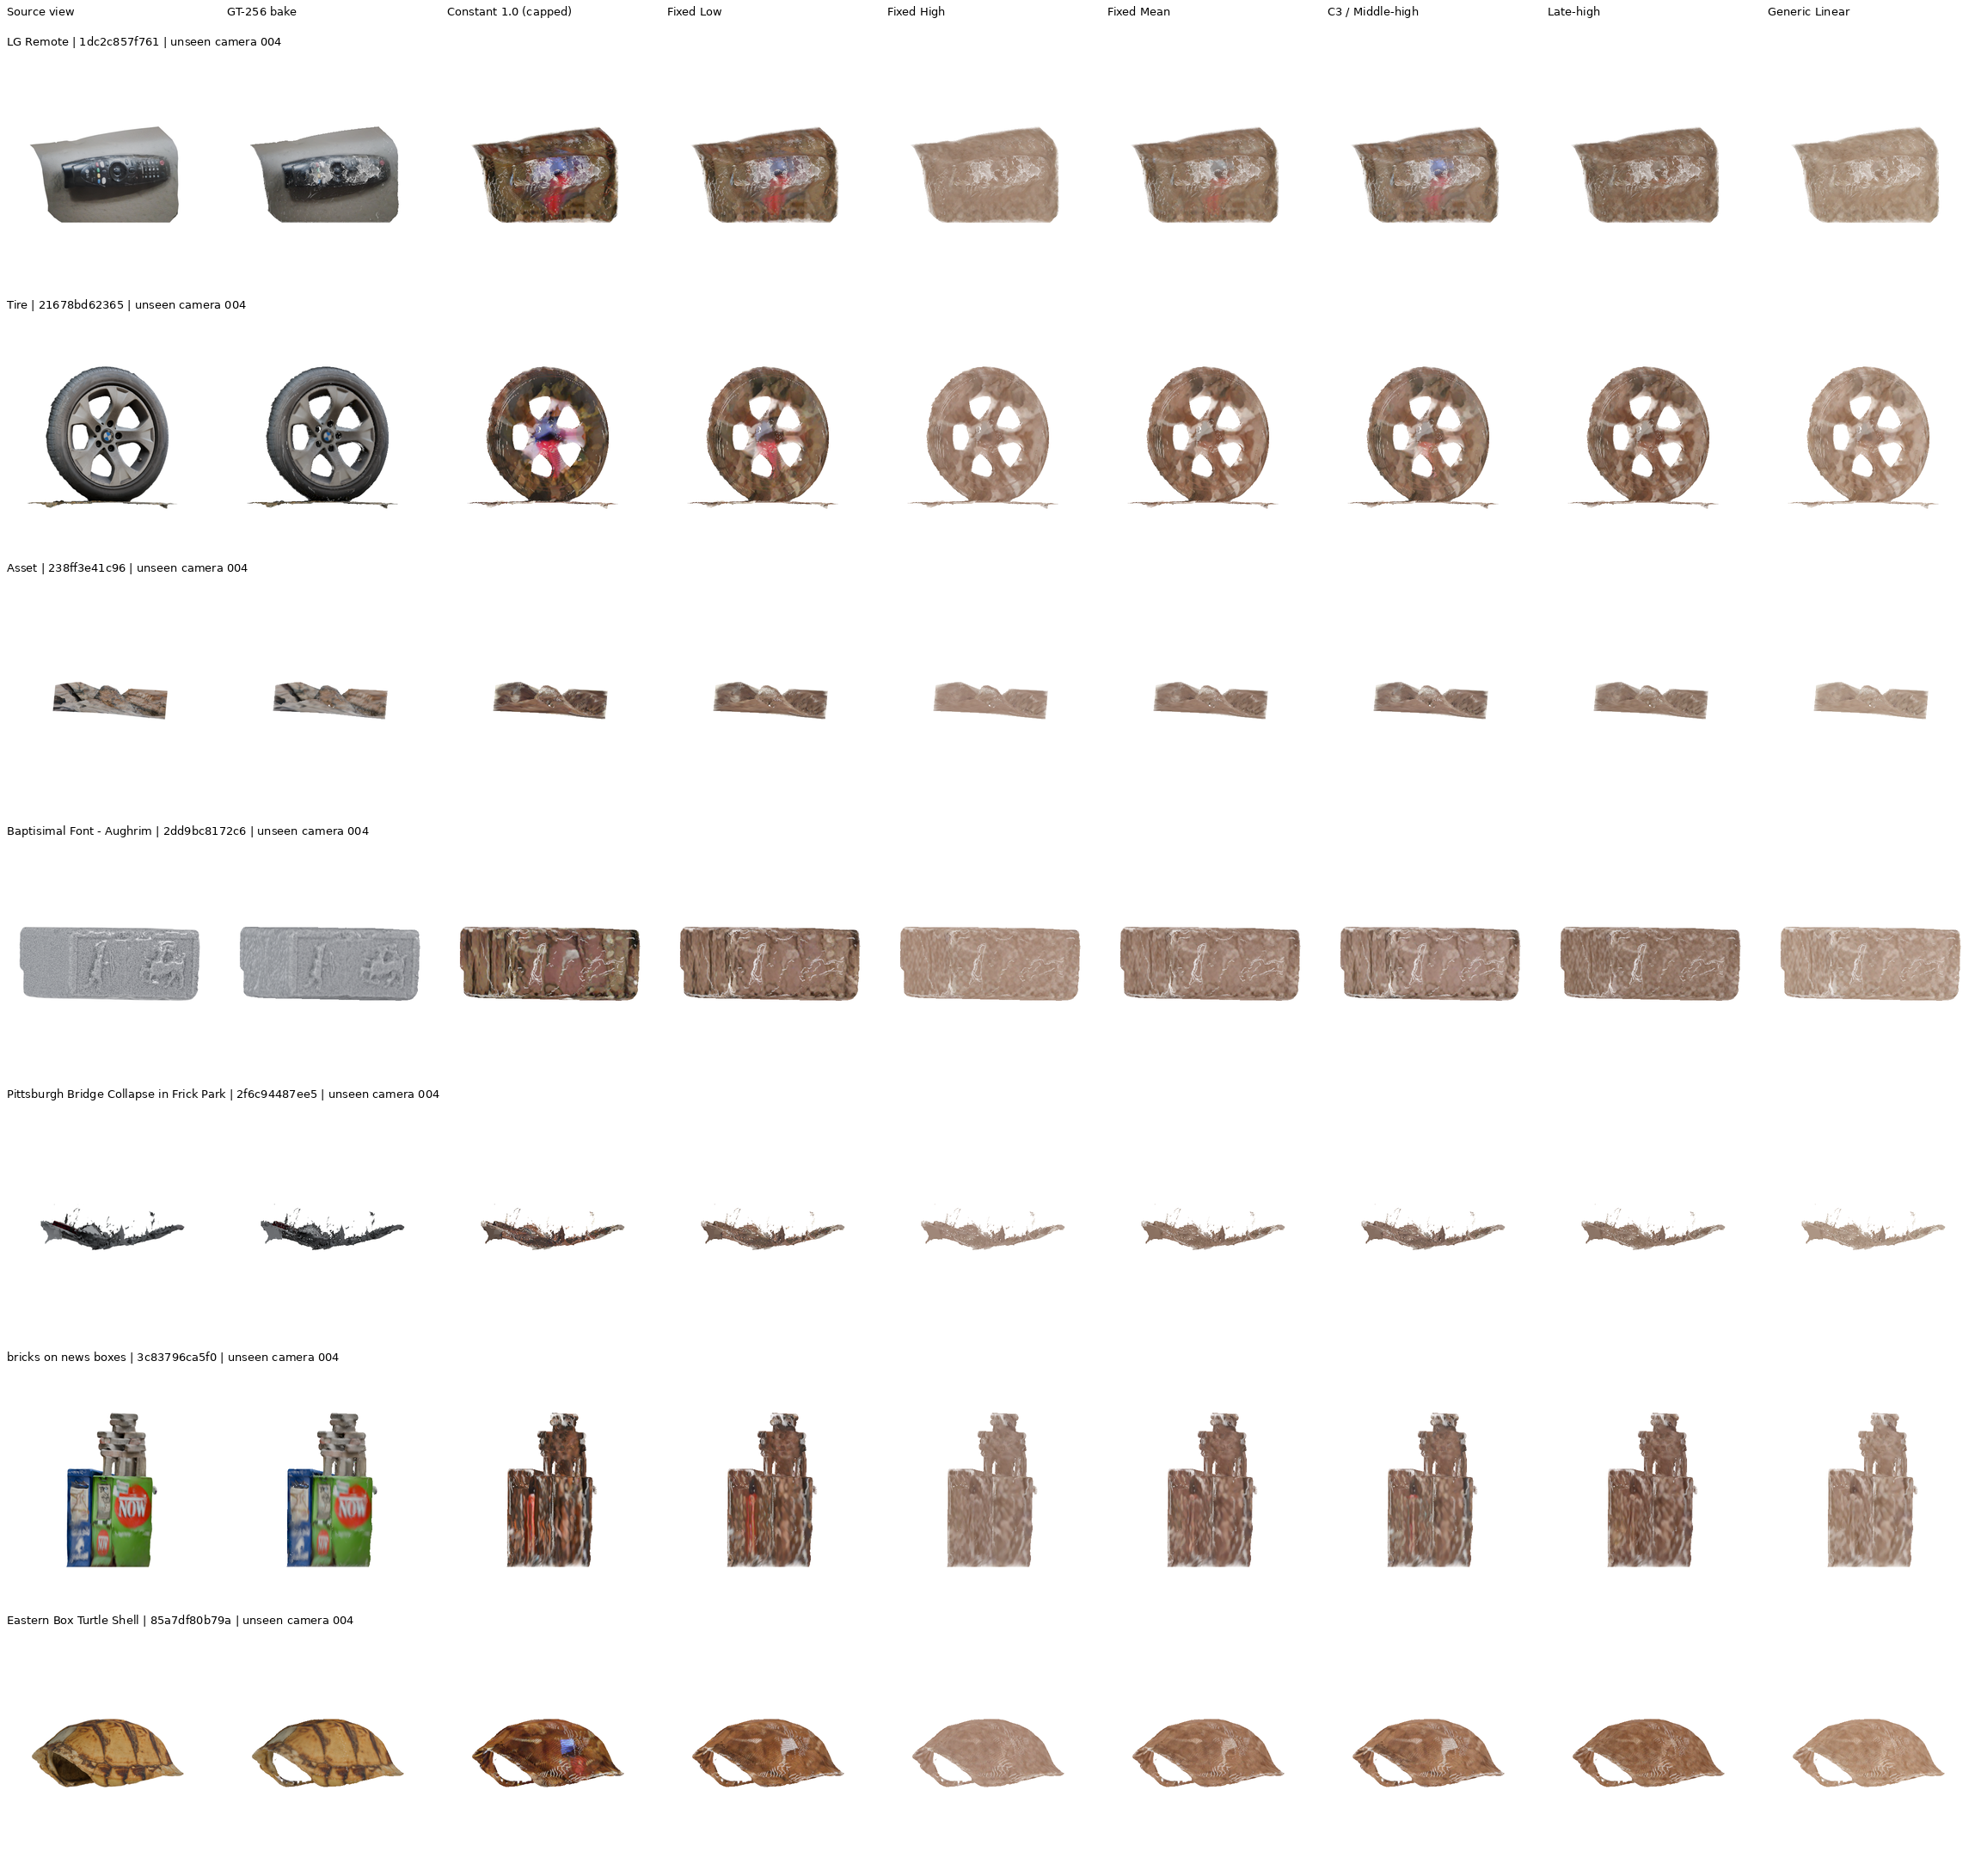
\includegraphics[width=\textwidth,height=0.84\textheight,keepaspectratio]{figures/figS2_baked_full_conditions.png}
\caption{Full-object same-camera source, GT-256 bake and all seven controls for the seven new-pilot objects whose publication licenses were verified. Three other objects remain in all numerical analyses but are omitted from distributed illustrations because image-publication permission is unresolved. No quality-based exclusion is made. Images are actual renders, resized for display without retouching. Source credits and input/output hashes are provided in BAKED\_ASSET\_CREDITS.csv and BAKED\_FIGURE\_VIDEO\_PROVENANCE.csv.}
\end{figure}

Supplementary Video presents two input-order, rights-cleared objects at all eleven discrete unseen cameras. Each actual rendered view is held for one second; no interpolated camera image is synthesized. It is an unlit comparison, not a claim of continuous-view or PBR quality.

LG Remote by mohd.akmal.mahyudin; CC Attribution. Source: \url{https://sketchfab.com/3d-models/1dc2c857f7614caeb6c2aa0559ccf973}.

Tire by Koto3D Stephane Vogley; CC Attribution. Source: \url{https://sketchfab.com/3d-models/21678bd623654182b52c11d013de4e71}.

Asset 238ff3e41c964655b83aa9c8770cc766 by suntaree; CC Attribution. Source: \url{https://sketchfab.com/3d-models/238ff3e41c964655b83aa9c8770cc766}.

Baptisimal Font - Aughrim by Galway3D\_DH\_AGe; CC0 Public Domain. Source: \url{https://sketchfab.com/3d-models/2dd9bc8172c6461797947cc7214db399}.

Pittsburgh Bridge Collapse in Frick Park by C8X; CC Attribution. Source: \url{https://sketchfab.com/3d-models/2f6c94487ee54cb88021f4643409d849}.

bricks on news boxes by bunnyhero; CC Attribution. Source: \url{https://sketchfab.com/3d-models/3c83796ca5f043f1beb8044dd2e51a0d}.

Eastern Box Turtle Shell by Frank McMains; CC Attribution. Source: \url{https://sketchfab.com/3d-models/85a7df80b79a4ba9b8c3a175de0dbce6}.


\clearpage
\section*{S19. Post hoc GT reference context and object influence}
This reanalysis uses the same valid ten-object source records and the same frozen endpoints; it is not a new holdout or a new confirmatory family. GT-256 is a matched empirical projection reference, not a theoretical upper bound on an image endpoint. Its mean PSNR/LPIPS/SSIM/Edge-SSIM/CIEDE2000 are 22.38/0.0590/0.7683/0.7533/4.44. Late-high's LPIPS gain relative to Fixed Mean is unchanged at 0.00265.

For descriptive magnitude context, the ratio of means is
\[
 r=\frac{\mathrm{mean}(\mathrm{LPIPS}_{Mean}-\mathrm{LPIPS}_{Late})}{\mathrm{mean}(\mathrm{LPIPS}_{Mean}-\mathrm{LPIPS}_{GT256})}=0.03720.
\]
The numerator and denominator are recomputed jointly in each of 50,000 object-bootstrap samples (seed 20261010). All bootstrap denominators are positive; the pointwise interval is [0.02275,0.05323]. This is a roughly 3.7\% reduction of the mean empirical reference gap, not evidence that the remaining appearance mismatch is small. It must not be interpreted as a practical acceptability threshold or a new primary discovery. Removing each object in turn yields Late--Mean mean differences between $-0.00294$ and $-0.00208$; this descriptive influence check does not create additional independent samples.

\begin{longtable}{lrrrr}
\caption{Same ten objects: matched reference and generated unseen-view FG-LPIPS. All eleven unseen views are averaged first. Full UIDs and exact values accompany the reanalysis script.}\\
\toprule UID prefix & GT-256 & Fixed Mean & Late-high & Late--Mean \\
\midrule\endfirsthead
\toprule UID prefix & GT-256 & Fixed Mean & Late-high & Late--Mean \\
\midrule\endhead
1dc2c857f761 & 0.07674 & 0.15307 & 0.14898 & -0.00408 \\
21678bd62365 & 0.07367 & 0.17198 & 0.16919 & -0.00279 \\
238ff3e41c96 & 0.02328 & 0.05895 & 0.05849 & -0.00046 \\
2dd9bc8172c6 & 0.14110 & 0.23763 & 0.22982 & -0.00781 \\
2f6c94487ee5 & 0.06525 & 0.09319 & 0.09317 & -0.00003 \\
3c83796ca5f0 & 0.05597 & 0.17757 & 0.17439 & -0.00318 \\
85a7df80b79a & 0.04051 & 0.10964 & 0.10519 & -0.00445 \\
e261c0fe85af & 0.04032 & 0.13280 & 0.13112 & -0.00168 \\
f1ccc55a65c7 & 0.06034 & 0.11759 & 0.11622 & -0.00137 \\
fa5c4b02c5b2 & 0.01312 & 0.05075 & 0.05010 & -0.00065 \\
\bottomrule\end{longtable}
The script \texttt{scripts/analyze\_gt\_context.py}, copied source CSV and \texttt{GT\_REFERENCE\_CONTEXT.json} permit standalone reproduction with NumPy. No generated output is added, replaced or retouched. The source hash identifies the previous round's valid metrics; historical five, N=20 and invalid old native-seven records remain separate.


\section*{S20. Native-wrapper controls and sampling-protocol scope}
The second iteration adds native-unset residual and No Adapter controls on the same ten objects, with no change to the earlier seven-condition matrix or its primary comparison. These objects and their earlier outcomes have been inspected, so all added contrasts are exploratory. The native control removes the scale attribute immediately before every actual wrapper invocation, leaving the original forward function, geometry features and reference-write skipping logic intact. A regenerated Constant 1.0 (capped) control matches the earlier RGB outputs bitwise on all ten objects; inputs and seeds also match. This identifies the default residual branch within the frozen protocol, not an unmodified complete pipeline.

A read-only source audit identifies additional differences. The frozen generator makes one conditional score prediction per denoising step, uses cached global image embeddings, and generates 256-pixel views. The full base-pipeline call defaults to 512-pixel views, online global embeddings, and classifier-free guidance of 2.0; its denoising loop combines conditional and unconditional predictions. The GeoTex model's validation call uses 75 steps and does not explicitly bind geometry features. Source differences alone cannot identify the cause of the appearance failures or validate a repair. The corresponding source hashes and audit assertions are delivered in \texttt{ITERATION002\_SAMPLING\_PROTOCOL\_AUDIT.json}.

\begin{figure}[htbp]
\centering
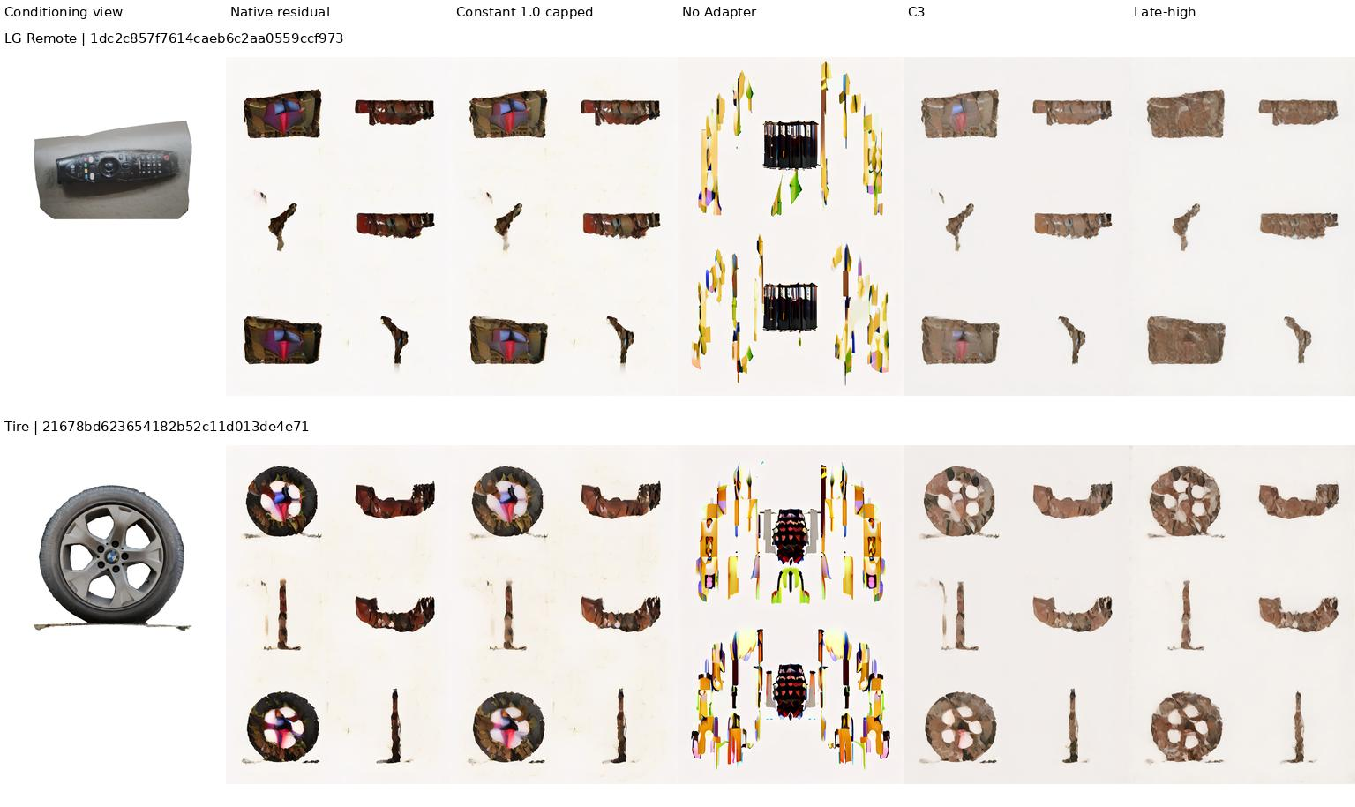
\includegraphics[width=\linewidth]{figures/figS3_native_controls.pdf}
\caption{Complete generated six-view grids for the same first two input-ordered, rights-cleared objects used in the earlier bake display. The conditioning image is shown separately. Native residual means the unset-scale wrapper branch in the frozen sampling protocol; it does not mean the complete default pipeline. All grids retain their original contents, with only whole-grid resizing; visible color and detail failures are not retouched. LG Remote: mohd.akmal.mahyudin; Tire: Koto3D Stephane Vogley; both CC Attribution. Full source links are given in S18; new output hashes and credits accompany this figure.}
\end{figure}


\subsection*{S20.1 Complete exploratory contrast family}
Each row is A minus Native residual. Higher PSNR/SSIM/Edge-SSIM and lower LPIPS/CIEDE2000 are favorable. The 95\% intervals are pointwise object-bootstrap intervals; adjusted $p$ values belong to one 15-test Holm family. All ten objects are retained, and eleven unseen views are averaged per object. The prior Late-high--Fixed Mean primary remains unchanged. Repeated GT metrics match the earlier evaluation exactly (maximum absolute difference 0).

\begin{table}[htbp]\centering\scriptsize
\begin{tabular}{llrrr}\toprule A & Endpoint & Mean difference & Pointwise 95\% CI & Holm $p$\\\midrule
Late-high & FG-PSNR & $+1.78764$ & $[+0.46170,+3.05975]$ & 0.29688 \\
Late-high & FG-LPIPS & $-0.00951$ & $[-0.01772,-0.00263]$ & 0.29688 \\
Late-high & FG-SSIM & $+0.08825$ & $[+0.05443,+0.12228]$ & 0.05469 \\
Late-high & Edge-SSIM & $+0.04958$ & $[+0.02256,+0.07663]$ & 0.12305 \\
Late-high & CIEDE2000 & $-4.82018$ & $[-8.66554,-0.65098]$ & 0.29688 \\
C3 & FG-PSNR & $+1.34525$ & $[+0.13241,+2.56138]$ & 0.29688 \\
C3 & FG-LPIPS & $-0.00699$ & $[-0.01326,-0.00159]$ & 0.29688 \\
C3 & FG-SSIM & $+0.06827$ & $[+0.04193,+0.09422]$ & 0.05469 \\
C3 & Edge-SSIM & $+0.03526$ & $[+0.01168,+0.05974]$ & 0.29688 \\
C3 & CIEDE2000 & $-4.30778$ & $[-7.73875,-0.53688]$ & 0.29688 \\
No Adapter & FG-PSNR & $-5.21580$ & $[-6.60353,-3.61839]$ & 0.05469 \\
No Adapter & FG-LPIPS & $+0.02281$ & $[+0.01287,+0.03317]$ & 0.05469 \\
No Adapter & FG-SSIM & $+0.04520$ & $[-0.02288,+0.11851]$ & 0.29688 \\
No Adapter & Edge-SSIM & $-0.21789$ & $[-0.26399,-0.16852]$ & 0.02930 \\
No Adapter & CIEDE2000 & $+14.44690$ & $[+6.37338,+22.12900]$ & 0.07812 \\
\bottomrule\end{tabular}
\caption{All added object-paired exploratory contrasts. These are previously inspected objects, not a new independent confirmation sample.}\end{table}
No Adapter versus Native residual Edge-SSIM is the sole adjusted rejection in this family. The favorable schedule means and pointwise intervals do not establish family-corrected schedule advantages or acceptable appearance fidelity. The generated-view controls also retain conspicuous color/detail failures in the displayed examples.


\section*{S21. Complete native base-pipeline diagnostic}
The third iteration uses the same two previously inspected, rights-cleared failure objects, not an independent confirmation cohort. We load the identical native base model assets directly, without GeoTex weights or geometry residuals, and call the complete pipeline at 50 and 75 steps. All four calls generate 1024$\times$1536 grids (six 512-pixel views). Observation hooks record exactly 50/75 actual UNet calls, each with the two-member classifier-free batch; the 50/75 starting latents match within each object. The scheduler is the native EulerAncestralDiscreteScheduler with trailing timesteps. The previously supplied batch conditioning hashes match, establishing source correspondence rather than full preprocessing equivalence.

The first RGB API attempt fails before any output because the native recenter helper expects four channels. It is preserved separately. The valid second attempt uses the original single-reference RGBA source. Native preprocessing mutates some white foreground pixels in place; the before/after input images are archived. Source inspection also identifies an incompatible validation entry in the GeoTex model: it wraps the UNet while the full pipeline's preparation entry asserts a bare UNet. This is a source-level finding, not a reported execution of the complete GeoTex validation path. Independent native base loading avoids that incompatibility without changing the pipeline's denoising code.

The frozen generator's image inverse scaling is $1.6x$, followed by $0.5x+0.5$, yielding $0.8x+0.5$. The full pipeline composes the same two factors. The formulas are algebraically equal; naming differences do not demonstrate a decoding error.

\begin{figure}[htbp]\centering
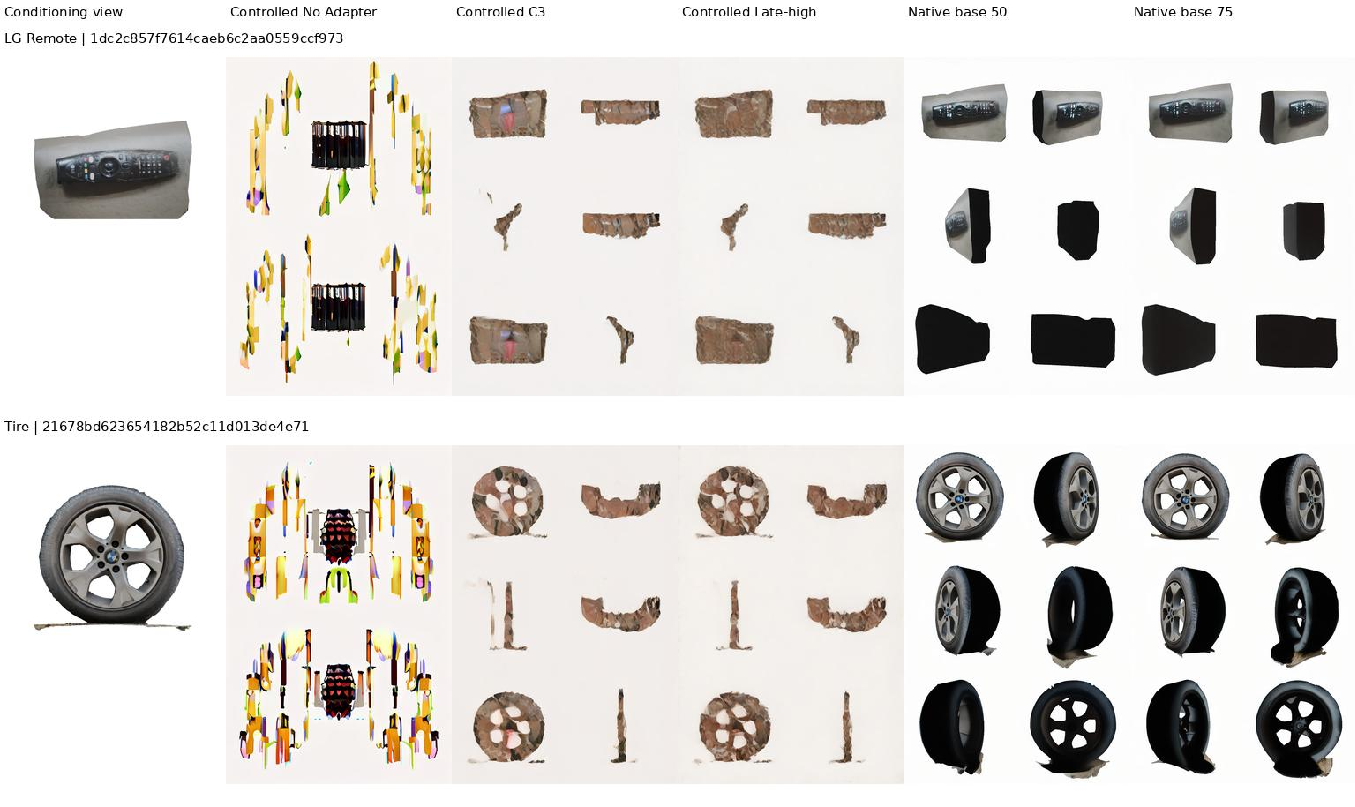
\includegraphics[width=\linewidth]{figures/figS4_native_base_diagnostic.pdf}
\caption{All generated views of two seen failure objects, with whole-grid resizing and no retouching. Native base columns use a different sampling protocol and unverified camera conventions; these panels are not aligned GT comparisons or complete GeoTex default results. Front-looking native outputs retain reference colors/details, while other views remain imperfect. Conditioning image is shown once; all four native calls are displayed, with no outcome selection. LG Remote: mohd.akmal.mahyudin; Tire: Koto3D Stephane Vogley; both CC Attribution, source links in S18. New hashes and credits accompany the figure.}
\end{figure}

The diagnostic justifies prioritizing a controlled separation of online/cached image features, classifier-free guidance and other sampling differences. It does not identify a single cause, establish a new algorithm, validate broad material fidelity or replace any earlier paired comparison. No inferential statistics or new acceptance probability are assigned to these two examples.


\section*{S22. Controlled guidance--image-feature diagnostic}
The same two seen failure objects undergo eight calls: cached/online global image features crossed with conditional-only/sequential CFG2, all without geometry residuals. Views remain 256 pixels, the sampler remains the frozen 50-step EulerDiscreteScheduler, and conditioning RGB/initial latent identities match the old control. Online encoders consume the same already processed conditioning RGB; native RGBA recentering and bright-pixel handling are not invoked. The online-to-cache feature cosines are 0.862997 for LG Remote and 0.899210 for Tire. Feature difference is not itself a fidelity measure or evidence of a bad cache.

The conditional-only arms reuse the original generation function. The cached arm reproduces both prior No Adapter RGB outputs bitwise. CFG2 uses the standard prediction $2\epsilon_c-\epsilon_u$ through sequential batch-one forwards. Negative conditioning encodes a zero tensor in the normalized VAE input space, with seed424242; its reference-noise call uses an independent RNG fork at each step (seed100042 plus step). The positive branch retains the original randomness: all fifty positive-call CUDA RNG states match across four arms for each object. Each guided arm records fifty positive and fifty negative calls; each conditional-only arm records fifty positive calls. This controlled sequential implementation is not claimed pixel-equivalent to the native batched CFG API.

\begin{figure}[htbp]\centering
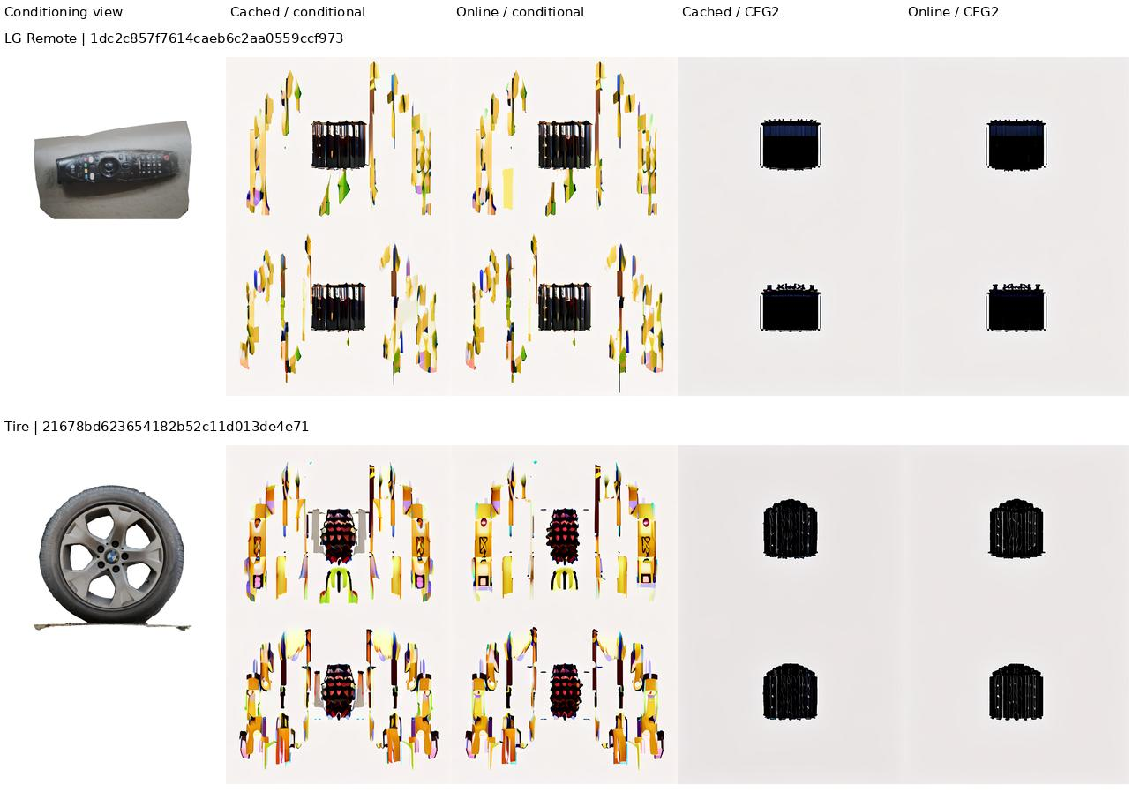
\includegraphics[width=\linewidth]{figures/figS5_guidance_embedding_factorial.pdf}
\caption{All eight six-view outputs from the frozen two-by-two diagnostic. Only whole-grid resizing is used. Online features do not restore reference appearance. Guided outputs lose much of the conspicuous colored pattern but retain incorrect dark shapes; this is not a demonstrated quality repair. Same previously inspected examples and rights as S21; all outputs, trace identities, hashes and credits are delivered.}
\end{figure}

No paired cross-camera GT endpoints, population tests or acceptance probability are assigned to these two examples. The result retains the earlier B2 feature-substitution failure and C1 visual-gate failure; it does not support erasing those records or claiming a validated appearance correction. Resolution and remaining full-pipeline differences should be separated before deploying an amended GeoTex path or developing a new method.


\section*{S23. Target-resolution bridge}
The two seen diagnostic objects undergo eight calls: 256/512-pixel target views crossed with conditional-only/sequential CFG2. Reference RGB resizing and model.img\_size remain 256; online global features, frozen model weights, 50-step EulerDiscrete sampling, training time IDs and reference encoding remain fixed. Initial latents have shape $1\times4\times96\times64$ or $1\times4\times192\times128$. Within each target resolution, the two arms use identical initial latents and fifty matching positive-call CUDA RNG states. Across resolutions, the tensor dimensions differ: a common seed is not a claim of identical initial tensors. Guided arms reuse the previous sequential CFG2 implementation and independent negative RNG policy.

Both 256-pixel arms reproduce the corresponding S22 online-feature RGB outputs bitwise for both objects. All conditions have identical reference-input and online-feature hashes within an object. Larger target grids change the object arrangement, but retained appearance defects prevent calling this a quality repair. Camera identities have not been independently calibrated across these generated grids, so there are no cross-path GT scores, population tests or deployment claims. The base pipeline source specifies a $1024\times1536$ output grid; this source fact and the controlled bridge motivate further protocol calibration, not retroactive pooling of different target resolutions.

\begin{figure}[htbp]\centering
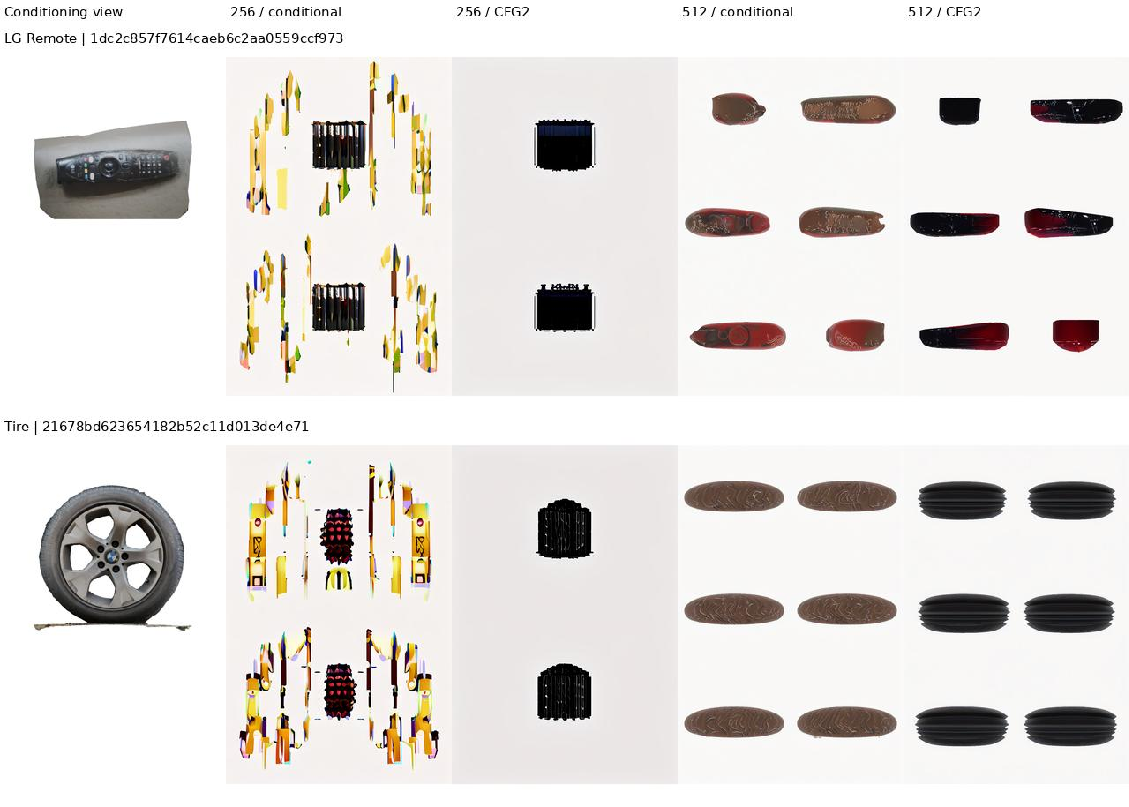
\includegraphics[width=\linewidth]{figures/figS6_target_resolution_bridge.pdf}
\caption{Eight complete outputs for the same seen, licensed examples, with whole-grid resizing only. The 512-pixel-view arms produce six-position arrangements while the 256-pixel-view controls retain malformed two-group structures. Colors, shape and fine details remain imperfect. This bounded diagnostic does not establish overall fidelity, correct camera labels or a working geometry-adapter deployment.}
\end{figure}


\section*{S24. Native geometry implementation and camera-contract audit}
The published inference source at commit \texttt{f714682db5e6f78e8d1c7c0a43d1525638dda5a6} arranges rendered indices $[0,5,1,4,2,3]$ in row-major order; its bake script extracts result tiles $[1,3,5,6,4,2]$, the inverse permutation. Actual metadata for all ten baking objects matches those nominal directions after the conditioning-camera anchor rotation. Pole elevation matches, but pole-image roll, cross-renderer pixel registration and generated-view fidelity remain unverified. The historical public training loader's repeated top view is separate from this inference contract. Source snapshots, hashes and the ten-object audit are provided.

Two seen objects first pass an identity gate: the frozen GeoTex weights are loaded, all geometry features cleared, and the full native pipeline outputs match the earlier bare-base RGB pixels exactly. The model constructor already wraps reference attention; setting its preparation state prevents double wrapping without replacing the native denoising loop.

The subsequent matrix has eight conditions per object: disabled, original unscaled residual, Fixed Low, Fixed High, Fixed Mean, C3, Late-high and Generic Linear. Native target views remain 512 pixels with CFG2 and fifty EulerAncestral steps; the trained geometry encoder input remains 256 pixels, with wrapper interpolation to actual hidden-state sizes. Historical schedule functions come from the frozen registry; Fixed Mean requests 1.65 and Late-high requests 1.25 except for the last sixteen steps at 2.50. Applied layer caps remain native. Historical C3's group-dependent profile does not share every layer budget with the scalar Fixed Mean; no equal-budget claim is made for that contrast.

Geometry features have batch one and broadcast to both batch-two CFG branches through hidden-state-dependent gates. All nine wrappers skip fifty reference-write corrections and execute fifty corrected read calls; each geometry-enabled correction has batch two and finite values. Within an object, geometry/input hashes, initial latents and the fifty outer-UNet CUDA RNG states match across all eight conditions. The disabled arm reproduces the previous bare native grid bitwise. The initial registry-import attempt failed before model loading because its required run configuration was absent; the failed source/record is retained, and the corrected attempt has a distinct output root.

\begin{figure}[htbp]\centering
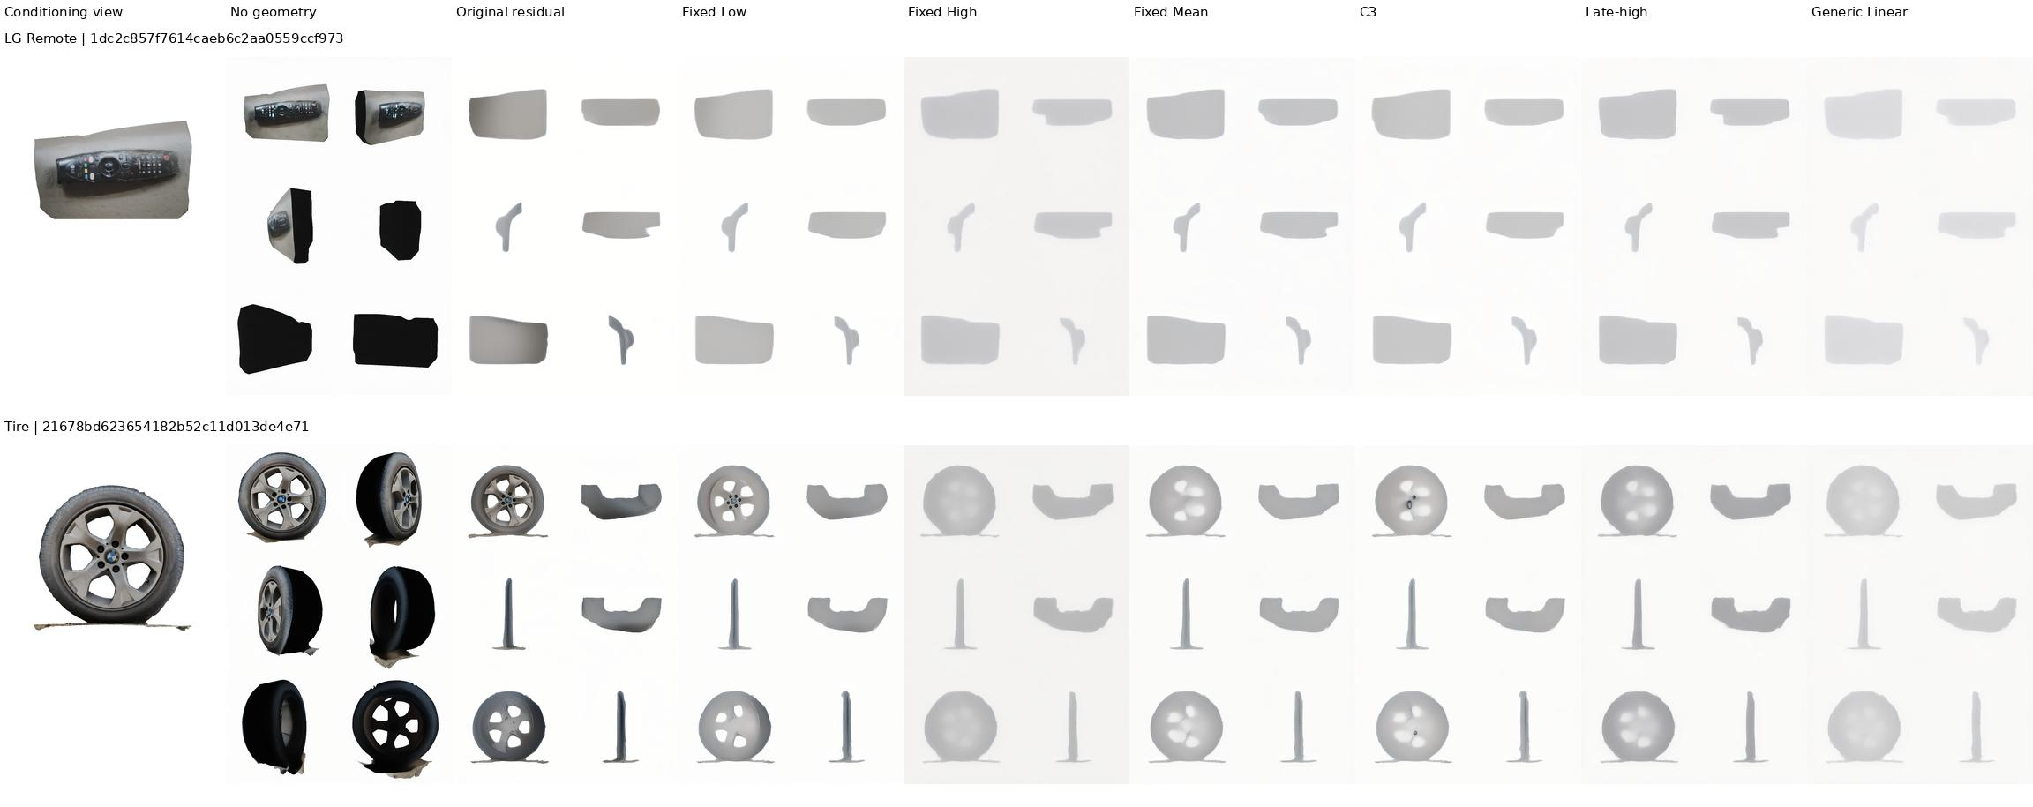
\includegraphics[width=\linewidth]{figures/figS7_native_geometry_matrix.pdf}
\caption{All sixteen complete native-loop outputs on the same two seen, licensed objects. Only full-grid display resizing is used. Geometry-enabled remote outputs lose most reference content; tire outputs retain some hub structure but several conditions blur it. Executable geometry control is not a demonstrated fidelity repair. Full-resolution images, observed wrapper counts, input/noise identities and credits accompany the figure.}
\end{figure}

These diagnostics are not an independent confirmation cohort, do not verify correct generated cameras and do not support population inference or cross-path GT statistics. They preserve the prior controlled and downstream results while restricting claims about native deployment. Geometry-encoding resolution and CFG-branch compatibility require further controlled examination.


\section*{S25. Geometry encoding, branch policy and recorded training audit}
The same two seen objects undergo twelve native-loop calls: geometry encoding at 256/512 pixels crossed with both-branch, conditional-only and conditional-only half-amplitude corrections. The native target grid, reference RGBA, online features, CFG2 and fifty EulerAncestral steps remain fixed. A controller acts after native correction computation: the both mode returns the correction unchanged; conditional-only zeros the negative sample; half-amplitude also multiplies the positive sample by 0.5. This is an implementation diagnostic, not a newly validated algorithm or a residual-dose-matched comparison. Half amplitude checks the conditional coefficient in CFG2; different trajectories prevent claiming equal total residual norms.

The 256/both output reproduces both S24 original-residual RGB grids bitwise. All nine wrappers retain fifty reference-write skips and fifty corrected reads. Input hashes, initial latents and outer-UNet RNG trajectories match within each object; geometry input/feature hashes match only within the same geometry encoding size. Every conditional-only read has zero negative correction norm. Complete output grids and trace identities are delivered.

\begin{figure}[htbp]\centering
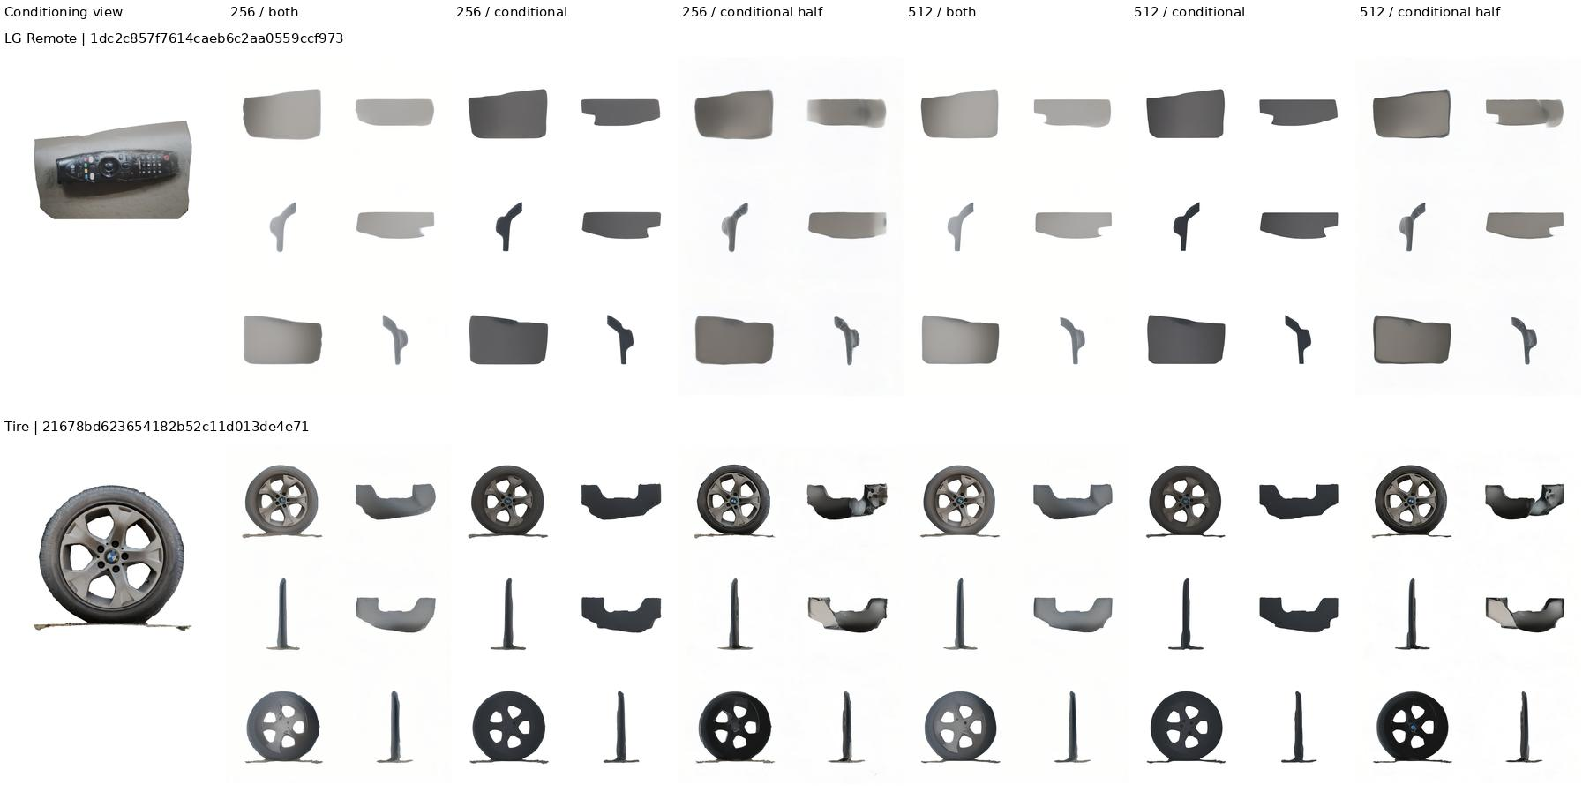
\includegraphics[width=\linewidth]{figures/figS8_encoding_branch_matrix.pdf}
\caption{All twelve full grids, resized only for display. Half-amplitude conditional corrections preserve more tire details, but remote reference content is still lost. Neither larger geometry encoding nor branch removal establishes an overall quality repair. Same previously inspected objects and attribution as S24.}
\end{figure}

The frozen checkpoint's recorded main-adapter training lineage includes a 1,118-object list, a matching checkpoint SHA256 and a complete 2,000-step loss CSV. The train list has no UID overlap with Fresh C; 1,112 objects have the six checked RGB/normal/depth input sets, and six have missing entries. These availability counts do not establish texture quality or authenticate each historical sampled object. The configuration specifies 256-pixel training and conditioning-drop probability 0.1, but the recorded custom training entry does not read that probability and uses only non-dropped conditioning. It bypasses the model-class training method. The historical dataset source has repeated-top target lists; the surviving dataset source differs from the recorded commit. Source and model-entry identities, the declared list override, checkpoint identity and current availability are audited separately.

Exact training replay remains unsupported: the transient list-override wrapper and training seed are not preserved, the CSV has no sampled-object identities, and the checkpoint contains adapter/encoder weights without an embedded step. A trailing literal newline escape in the original manifest is preserved and explicitly handled rather than silently rewriting that artifact. This audit concerns the current main-adapter lineage, not restoration of the historical FAC branch. Conditional-only training explains why unrestricted negative-branch insertion needs validation, but the controlled outputs do not establish it as the sole cause of appearance loss. No independent generalization or cross-camera GT inference is made.


\section*{S26. Native training preflight and frozen new-training protocol}
The recorded custom trainer's shortcomings motivate a new main-adapter training protocol; this is not a FAC retraining or a replay of the historical pooled result. Of 1118 recorded training UIDs, six lack required inputs. Strict evaluation of the remaining 1112 retains 1090 and lists 22 input failures before any output-quality assessment. The old loader's random replacement of a failed object is disabled. The retained cohort has zero UID overlap with the 300 Fresh C objects. Geometry and target views are 512 pixels, use unique6 ordering, and have fixed resize ratio 1.0. Native reference preprocessing is captured from the actual pipeline at its first UNet call, including positive and negative CLIP embeddings, reference latents and added time IDs; these cached inputs are not generated evaluation outputs.

Three zero-valued depth channels in a real training object formerly produced a non-finite inverse-depth normalization. Values that cannot be inverted are encoded using the existing invalid-depth value before inversion; source RGB and normal maps are unchanged. This guard does not establish the physical meaning of those zero values. A separate precision probe finds all nine initial residual tensors nonzero, but their half-precision mean squares underflow to zero; float32 evaluation gives positive means of order $10^{-8}$. The new loss evaluates this term before clearing the wrapper records. Neither observation is used to claim a single cause of the historical quality failure.

Two scale-zero native outputs are pixel-identical to the preceding bare-base outputs. Captured conditions for the first two training UIDs are identical across the two GPUs. Two actual single-GPU optimizer steps, one conditional and one unconditional, produce finite nonzero gradients in both the adapters and geometry encoder, change their weight hashes, and use about 12.6 GB peak allocated memory. Smoke weights are discarded. A separate two-rank backward gate confirms finite gradients for all active parameters and synchronized updates. The unused projected x1 branch is frozen in the up-only architecture while its weights remain stored; 2,201,760 parameters remain active.

The formal protocol freezes 2000 successful optimizer updates, two GPUs with one object each per update, AdamW learning rate $10^{-4}$ and weight decay 0.01, gradient clipping at 1.0, initialization seed 42, and actual Bernoulli conditioning dropout probability 0.1. Positive/negative native conditioning is selected by the realized dropout flag. The base denoiser remains frozen. Object order, noise step, dropout, loss terms, gradient scale and gradient norm are logged per rank. Checkpoints are stored every 500 updates, and the final step-2000 checkpoint is specified in advance rather than selected on output quality. The global batch differs from the historical single-object trainer; this is a new protocol and does not isolate any one training change. The fixed 2000 updates have now completed on both ranks, with 4000 total object exposures; realized conditioning-drop fractions are 0.0920 and 0.1085. A completion audit reproduces the seeded object order and dropout flags, verifies synchronized finite gradients and optimizer steps, and records the final checkpoint hash. No new checkpoint quality result is claimed before the frozen native-path evaluation finishes. Packaged preflight records permit integrity and cohort checks; rerunning GPU execution additionally requires the recorded base assets, rendered training data and software environment.


\section*{S27. Complete new training and full-native baseline identity audit}
The new main-adapter training uses the frozen local hf\_repo UNet; its completion does not make it an official default-model replay. A read-only asset audit finds that the local converted v29 checkpoint includes 1680 UNet tensors and 863 ControlNet keys, and that the hf\_repo UNet differs from the v29 custom UNet even after casting to the same precision. Thus the preceding bare-base controls identify the native inference loop with the stated frozen HF assets, not the complete official default weights and ControlNet pipeline. These differences are retained rather than changing the historical source assets or treating them as a single established cause of the observed appearance failures.

A CPU audit strictly loads all 2543 full-checkpoint keys into the official ControlNet architecture with matching shapes and values; the ControlNet branch has 1,254,646,800 parameters. This establishes local asset compatibility, not GPU execution, canonical remote checkpoint byte identity or deployment quality. A matched 50-step, seed-42 comparison would differ from the official command-line defaults of 75 steps, seed 12 and background removal; those settings must be named explicitly. Input, architecture or weight-identity checks alone do not prove image quality. The new checkpoint's fifty-object cohort and object-level tests were frozen before viewing its outputs; inherited Fresh C exposure, nominal camera-direction limits and the absence of a FAC historical replay remain explicit.
\end{document}

